\documentclass{ximera}

\begin{document}
	\author{Stitz-Zeager}
	\xmtitle{TITLE}


\mfpicnumber{1}

\opengraphsfile{TheCircularFunctionsSineandCosine}

\setcounter{footnote}{0}

\label{TheCircularFunctionsSineandCosine}

In Section \ref{circularmotion}, we introduced circular motion and derived a formula which describes the linear velocity of an object moving on a circular path at a constant angular velocity.  One of the goals of this section is describe the \textit{position} of such an object.  To that end, consider an angle $\theta$ in standard position and let $P$ denote the point where the terminal side of $\theta$ intersects the Unit Circle, as diagrammed below.

\smallskip

\begin{tabular}{cc}

\begin{mfpic}[20]{-5}{5}{-5}{5}
\axes
\tlabel(4.75,-0.5){\scriptsize $x$}
\tlabel(0.25,5){\scriptsize $y$}
\tlabel(3.1,-0.75){\scriptsize $1$}
\tlabel(0.25,3.1){\scriptsize $1$}
\xmarks{-3 step 3 until 3}
\ymarks{-3 step 3 until 3}
\point[4pt]{(0,0)}
\drawcolor[gray]{0.7}
\circle{(0,0),3}
\drawcolor{black}
\arrow \parafcn{5, 55, 5}{1.5*dir(t)}
\penwd{1.25pt}
\arrow \reverse \arrow \polyline{(5,0),(0,0), (2.5, 4.3301)}

\tlabel[cc](1.9, 1){$\theta$}
\end{mfpic} 

&

\hspace{.25in}

\begin{mfpic}[20]{-5}{5}{-5}{5}
\axes
\tlabel(4.75,-0.5){\scriptsize $x$}
\tlabel(0.25,5){\scriptsize $y$}
\tlabel(3.1,-0.75){\scriptsize $1$}
\tlabel(0.25,3.1){\scriptsize $1$}
\xmarks{-3 step 3 until 3}
\ymarks{-3 step 3 until 3}
\arrow \reverse \arrow \polyline{(5,0),(0,0), (2.5, 4.3301)}
\tlabel(2,2.6){$P(\cos(\theta), \sin(\theta))$}
\drawcolor[gray]{0.7}
\circle{(0,0),3}
\drawcolor{black}
\arrow \parafcn{5, 55, 5}{1.5*dir(t)}
\penwd{1.25pt}
\arrow \reverse \arrow \polyline{(5,0),(0,0), (2.5, 4.3301)}
\tlabel[cc](1.9, 1){$\theta$}
\point[4pt]{(0,0), (1.5, 2.5981)}
\end{mfpic} 

\end{tabular}

\smallskip

 By associating the point $P$ with the angle $\theta$, we are assigning a \emph{position} on the Unit Circle to the angle $\theta$.  Since for each angle $\theta$, the terminal side of $\theta$, when graphed in standard position, intersects The Unit Circle only once, the mapping of $\theta$ to $P$ is a function.\footnote{See Definition \ref{functiondefn} in Section \ref{FunctionsandtheirRepresentations}.}   Since there is only \textit{one} way to describe a point using rectangular coordinates,\footnote{See page \pageref{importantfactscartesianplane} in Section \ref{AppCartesianPlane}.}  the mappings of $\theta$ to each of the $x$ and $y$ coordinates of $P$ are also functions.  We give these functions names in the following definition.
 
 \smallskip
 
 \colorbox{ResultColor}{\bbm

\begin{defn} \label{sinecosineunitcircledefn}  Suppose an angle $\theta$ is graphed in standard position. Let $P(x,y)$ be the point of intersection of the terminal side of $P$ and the Unit Circle.  

\begin{itemize}

\item The $x$-coordinate of $P$ is called the \index{cosine ! of an angle} \textbf{cosine} of $\theta$, written $\cos(\theta)$.

\item The $y$-coordinate of $P$ is called the \index{sine ! of an angle} \textbf{sine} of $\theta$, written $\sin(\theta)$.\footnote{The etymology of the name `sine' is quite colorful, and the interested reader is invited to research it;  the `co' in `cosine' is related to the concept of `co'mplementary angles (see Sections \ref{AppAngles} and \ref{AppRightTrig}) and is explained in detail in Section \ref{MoreTrigonometricIdentities}.} 

\end{itemize}

\end{defn}

\ebm} 
 
 
\smallskip

You may have already seen definitions for the sine and cosine of an (acute) angle  in terms of ratios of sides of a right triangle.\footnote{For instance, Definition \ref{righttrianglesinecosinetangent} in Section \ref{AppRightTrig}.}  While not incorrect, defining sine and cosine using right triangles limits the angles we can study to acute angles only.  Definition \ref{sinecosineunitcircledefn}, on the other hand, applies to \textit{all} angles. Since these functions are defined in terms of points on the Unit \textit{Circle}, they are called \index{circular functions}\index{functions ! circular} \textbf{circular} functions.  Rest assured,  Definition \ref{sinecosineunitcircledefn} specializes to Definition \ref{righttrianglesinecosinetangent} when $\theta$ is an acute angle.  We will see instances of this fact in the next example.


\begin{ex} \label{cosinesineviaunitcircle}  Find the sine and cosine of the following angles.

\begin{multicols}{5}

\begin{enumerate}

\item  $\theta = 270^{\circ}$

\item $\theta = - \pi$

\item  $\theta = 45^{\circ}$

\item  $\theta = \frac{\pi}{6}$

\item  $\theta = \frac{5\pi}{6}$ \label{refangleintro}

\end{enumerate}

\end{multicols}

{\bf Solution.}

\begin{enumerate}

\item  To find $\cos\left(270^{\circ}\right)$ and $\sin\left(270^{\circ}\right)$, we plot the angle $\theta =270^{\circ}$ in standard position and find the point on the terminal side of $\theta$ which lies on the Unit Circle.  Since $270^{\circ}$ represents $\frac{3}{4}$ of a counter-clockwise revolution, the terminal side of $\theta$ lies along the negative $y$-axis.  Hence, the point we seek is $(0,-1)$ so that  $\cos\left(270^{\circ}\right) = 0$ and $\sin\left(270^{\circ}\right) = -1$.

\item  The angle $\theta=-\pi$ represents one half of a clockwise revolution so its terminal side lies on the negative $x$-axis.  The point on the Unit Circle that lies on the negative $x$-axis is $(-1,0)$ which means  $\cos(-\pi) = -1$ and $\sin(-\pi) = 0$.

\begin{tabular}{cc}

\begin{mfpic}[18]{-5}{5}{-5}{5}
\axes
\tlabel(4.75,-0.5){\scriptsize $x$}
\tlabel(0.25,5){\scriptsize $y$}
\tlabel(3.1,-0.75){\scriptsize $1$}
\tlabel(0.25,3.1){\scriptsize $1$}
\tcaption{Finding $\cos\left(270^{\circ}\right)$ and $\sin\left(270^{\circ}\right)$}
\xmarks{-3 step 3 until 3}
\ymarks{-3 step 3 until 3}
\tlabel(0.25,-3.75){$P(0, -1)$}
\drawcolor[gray]{0.7}
\circle{(0,0),3}
\drawcolor{black}
\arrow \parafcn{5, 265, 5}{1.5*dir(t)}
\penwd{1.25pt}
\arrow \reverse \arrow \polyline{(5,0), (0,0), (0,-5)}
\tlabel(-2, 1.75){\scriptsize $\theta = 270^{\circ}$}
\point[4pt]{(0,0), (0, -3)}
\end{mfpic} 

&

\hspace{0.25in}

\begin{mfpic}[18]{-5}{5}{-5}{5}
\axes
\tlabel(4.75,-0.5){\scriptsize $x$}
\tlabel(0.25,5){\scriptsize $y$}
\tlabel(3.1,-0.75){\scriptsize $1$}
\tlabel(0.25,3.1){\scriptsize $1$}
\tcaption{Finding $\cos\left(-\pi\right)$ and $\sin\left( -\pi \right)$}
\xmarks{-3 step 3 until 3}
\ymarks{-3 step 3 until 3}
\tlabel(-5.5,0.5){$P(-1, 0)$}
\drawcolor[gray]{0.7}
\circle{(0,0),3}
\drawcolor{black}
\arrow \parafcn{-5, -175, -5}{1.5*dir(t)}
\penwd{1.25pt}
\arrow \reverse \arrow \polyline{(-5,0), (5,0)}
\tlabel[cc](1, -2){\scriptsize $\theta=-\pi$}
\point[4pt]{(0,0), (-3, 0)}
\end{mfpic} 

\end{tabular}

\item  In  Section \ref{AppRightTrig}, we derived values for $\cos\left(45^{\circ}\right)$ and $\sin\left(45^{\circ}\right)$ using  Definition \ref{righttrianglesinecosinetangent}.  In order to connect what we know from   Section \ref{AppRightTrig} with what we are asked to find per  Definition \ref{sinecosineunitcircledefn}, we sketch $\theta = 45^{\circ}$ in standard position and let $P(x,y)$ denote the point on the terminal side of $\theta$ which lies on the Unit Circle.  If we drop a perpendicular line segment from $P$ to the $x$-axis as shown below on the left,  we obtain a $45^{\circ} - 45^{\circ} - 90^{\circ}$ right triangle whose legs have lengths $x$ and $y$ units with hypotenuse $1$. From our work in Section \ref{AppRightTrig}, we obtain the (familiar) values $x = \cos\left(45^{\circ}\right) = \frac{\sqrt{2}}{2}$ and $y = \sin\left(45^{\circ}\right) = \frac{\sqrt{2}}{2}$.
\medskip


\item  As before, the terminal side of $\theta = \frac{\pi}{6}$ does not lie on any of the coordinate axes, so we proceed using a triangle approach.  Letting $P(x,y)$ denote the point on the terminal side of $\theta$ which lies on the Unit Circle, we drop a perpendicular line segment from $P$ to the $x$-axis to form a $30^{\circ} - 60^{\circ} - 90^{\circ}$ right triangle.   Re-using some of our work from Section \ref{AppRightTrig}, we get $x = \cos\left(\frac{\pi}{6}\right) = \frac{\sqrt{3}}{2}$ and $y=\sin\left(\frac{\pi}{6}\right) = \frac{1}{2}$. 

\begin{tabular}{m{2.5in}m{1in}m{2.5in}}

\begin{mfpic}[18]{-5}{5}{-5}{5}
\axes
\tlabel(4.75,-0.5){\scriptsize $x$}
\tlabel(1.4,-0.5){\scriptsize $x$}
\tlabel(0.25,5){\scriptsize $y$}
\tlabel(3,1.4){\scriptsize $y$}
\tlabel(4.1,-1){\scriptsize $1$}
\tlabel(0.25,4.1){\scriptsize $1$}
\tlabel(1.4,2){\scriptsize $1$}
\xmarks{-4 step 4 until 4}
\ymarks{-4 step 4 until 4}
\tlabel(3.5,2.5){$P(x,y)$}
\drawcolor[gray]{0.7}
\circle{(0,0),4}
\drawcolor{black}
\arrow \parafcn{5, 35, 5}{dir(t)}
\tlabel(1.15, .5){\scriptsize $\theta =  45^{\circ}$}
\point[4pt]{(0,0), (2.8284, 2.8284)}
\dashed \polyline{(2.8284, 2.8284), (2.8284, 0)}
\polyline{(2.5284, 0), (2.5284, 0.3), (2.8284, 0.3)}
\penwd{1.25pt}
\arrow \reverse \arrow \polyline{(5,0),(0,0), (3.5355, 3.5355)}

\end{mfpic} 

&

&

\begin{mfpic}[18]{-5}{5}{-5}{5}
\axes
\tlabel(4.75,-0.5){\scriptsize $x$}
\tlabel(1.7,-0.5){\scriptsize $x$}
\tlabel(0.25,5){\scriptsize $y$}
\tlabel(3.6,0.8){\scriptsize $y$}
\tlabel(4.1,-1){\scriptsize $1$}
\tlabel(0.25,4.1){\scriptsize $1$}
\tlabel(1.7,1.25){\scriptsize $1$}
\xmarks{-4 step 4 until 4}
\ymarks{-4 step 4 until 4}
\tlabel(3.75,1.70){$P(x,y)$}
\drawcolor[gray]{0.7}
\circle{(0,0),4}
\drawcolor{black}
\arrow \parafcn{5, 25, 5}{1.5*dir(t)}
\point[4pt]{(0,0), (3.4641, 2)}
\dashed \polyline{(3.4641,2), (3.4641, 0)}
\polyline{(3.1641, 0), (3.1641, 0.3), (3.4641, 0.3)}
\penwd{1.25pt}
\arrow \reverse \arrow \polyline{(5,0),(0,0), (4.330,2.5)}
\tlabel(1.75, .25){\scriptsize $\theta =  \frac{\pi}{6}$}
\end{mfpic} 

\end{tabular}


\item  We plot $\theta = \frac{5\pi}{6}$ in standard position below on the left  and, as usual, let $P(x,y)$ denote the point on the terminal side of $\theta$ which lies on the Unit Circle.  In plotting $\theta$, we find it lies $\frac{\pi}{6}$ radians short of one half revolution. Since we've just determined that $\cos\left(\frac{\pi}{6}\right) = \frac{\sqrt{3}}{2}$ and $\sin\left( \frac{\pi}{6} \right) = \frac{1}{2}$, we know  the coordinates of the point $Q$ below on the right are $\left(\frac{\sqrt{3}}{2}, \frac{1}{2}\right)$.  Using symmetry, the coordinates of $P$ are $\left(-\frac{\sqrt{3}}{2}, \frac{1}{2}\right)$, so $\cos\left(\frac{5\pi}{6}\right) = -\frac{\sqrt{3}}{2}$ and $\sin\left( \frac{5\pi}{6} \right) = \frac{1}{2}$.


\begin{tabular}{cc}


\begin{mfpic}[18]{-5}{5}{-5}{5}
\axes
\tlabel(4.75,-0.5){\scriptsize $x$}
\tlabel(0.25,5){\scriptsize $y$}
\tlabel(4.1,-1){\scriptsize $1$}
\tlabel(0.25,4.1){\scriptsize $1$}
\xmarks{-4 step 4 until 4}
\ymarks{-4 step 4 until 4}
\tlabel(-5.25,1.70){\scriptsize $P(x,y)$}
\drawcolor[gray]{0.7}
\circle{(0,0),4}
\drawcolor{black}
\arrow \parafcn{5, 145, 5}{1.5*dir(t)}
\arrow \reverse \arrow \parafcn{155, 175, 5}{1.5*dir(t)}
\tlabel(1, 1.75){\scriptsize $\theta =  \frac{5\pi}{6}$}
\tlabel(-2.5, .25){\scriptsize $\frac{\pi}{6}$}
\point[4pt]{(0,0), (-3.4641, 2)}
\penwd{1.25pt}
\arrow \reverse \arrow \polyline{(5,0),(0,0), (-4.330,2.5)}
\end{mfpic} 

&

\hspace{.5in}

\begin{mfpic}[18]{-5}{5}{-5}{5}
\axes
\tlabel(4.75,-0.5){\scriptsize $x$}
\tlabel(0.25,5){\scriptsize $y$}
\tlabel(4.1,-1){\scriptsize $1$}
\tlabel(0.25,4.1){\scriptsize $1$}
\xmarks{-4 step 4 until 4}
\ymarks{-4 step 4 until 4}
\tlabel(3.75,1.70){\scriptsize $Q\left(\frac{\sqrt{3}}{2}, \frac{1}{2}\right)$}
\tlabel(-6.25,1.70){\scriptsize $P\left(-\frac{\sqrt{3}}{2}, \frac{1}{2}\right)$}
\drawcolor[gray]{0.7}
\circle{(0,0),4}
\drawcolor{black}
\dotted  \polyline{(0,0), (4.330,2.5)}
\dotted \polyline{(-3.4641, 2), (3.4641, 2)}
\arrow \parafcn{5, 25, 5}{2*dir(t)}
\arrow \reverse \arrow \parafcn{155, 175, 5}{1.5*dir(t)}
\tlabel(2.25, .25){\scriptsize $\frac{\pi}{6}$}
\tlabel(-2.5, .25){\scriptsize $\frac{\pi}{6}$}
\arrow \parafcn{5, 145, 5}{1.5*dir(t)}
\tlabel(.75, 1.3){\scriptsize $\theta = \frac{5 \pi}{6}$}
\point[4pt]{(0,0), (3.4641, 2), (-3.4641, 2) }

\penwd{1.25pt}
 \arrow \reverse \arrow \polyline{(5,0),(0,0), (-4.330,2.5)}
\end{mfpic} 

\end{tabular}


  \qed

\end{enumerate}

\end{ex}

A few remarks are in order.  First, after having re-used some of our work from Section \ref{AppRightTrig} in a few specific instances, we can reconcile Definition \ref{sinecosineunitcircledefn} with Definition \ref{righttrianglesinecosinetangent} in the case $\theta$ is an acute angle.  We situate $\theta$ in a right triangle with hypotenuse length $1$, adjacent side length `$x$,' and the opposite side length `$y$' as seen below on the left. Placing the vertex of $\theta$ at the origin and the adjacent side of $\theta$ along the $x$-axis as seen below on the right effectively puts $\theta$ in standard position with $\theta$'s adjacent side as the initial side of $\theta$ and the hypotenuse  as the terminal side of $\theta$.  Since the hypotenuse of the triangle has length $1$, we know the point $P(x,y)$ is on the Unit Circle.\footnote{Do you see why?}

 \begin{tabular}{m{2.5in}m{0.5in}m{2.5in}}

\begin{mfpic}[15]{-5}{5}{-5}{5}
\arrow \reverse \arrow \shiftpath{(-4.330,0)} \parafcn{5, 25, 5}{3*dir(t)}
\polyline{(3.93, 0), (3.93, 0.4), (4.33, 0.4)}
\penwd{1.25pt}
\polyline{(-4.330,0), (4.330,0), (4.330,5), (-4.330,0)}
\tlabel(-1, 0.6){$\theta$}
\tlabel(0,-0.75){$x$}
\tlabel(4.75,2.25){$y$}
\tlabel(0,3){$1$}

\end{mfpic}
&

&

\begin{mfpic}[15]{-5}{5}{-5}{5}
\axes
\tlabel(4.75,-0.5){\scriptsize $x$}
\tlabel(0.25,4.75){\scriptsize $y$}
\tlabel(1.7,-0.5){\scriptsize $x$}
\tlabel(3.6,0.65){\scriptsize $y$}
\tlabel(4.1,-1){\scriptsize $1$}
\tlabel(0.25,4.1){\scriptsize $1$}
\xmarks{-4 step 4 until 4}
\ymarks{-4 step 4 until 4}
\tlabel(3.75,1.60){\scriptsize $P(x,y)$}
\drawcolor[gray]{0.7}
\circle{(0,0),4}
\drawcolor{black}
\arrow \parafcn{5, 25, 5}{1.5*dir(t)}
\tlabel(1.75, .25){\scriptsize $\theta$}
\point[4pt]{(0,0), (3.4641, 2)}
\polyline{(3.4641,2), (3.4641, 0)}
\polyline{(3.1641, 0), (3.1641, 0.3), (3.4641, 0.3)}
\penwd{1.25pt}
\arrow \reverse \arrow \polyline{(5,0),(0,0), (4.330,2.5)}

\end{mfpic} 

\end{tabular}

Definition \ref{righttrianglesinecosinetangent} gives $\cos(\theta) = \frac{x}{1} = x$ and $\sin(\theta) = \frac{y}{1} = y$ which exactly matches Definition \ref{sinecosineunitcircledefn}.  Hence, in the case of acute angles, the two definitions agree. In other words,  the values of the \textit{trigonometric ratios} of acute angles are the same as the corresponding \textit{circular function} values. 

\smallskip
 
A second important take-away from Example \ref{cosinesineviaunitcircle} is use of symmetry in  number \ref{refangleintro}.  Indeed, we found the sine and cosine of $\frac{5\pi}{6}$ using  the (acute) angle $\frac{\pi}{6}$ `for reference.'   Since the Unit Circle is rife with symmetry, we would like to generalize this concept and exploit symmetry whenever possible.  To that end, we introduce the notion of \index{angle ! reference}\index{reference angle}\textbf{reference angle}.

\smallskip

In general, for a non-quadrantal angle $\theta$, the reference angle for $\theta$ (which we'll usually denote $\alpha$) is the \textit{acute} angle made between the terminal side of $\theta$ and the $x$-axis.  If $\theta$ is a Quadrant I or IV angle, $\alpha$ is the angle between the terminal side of $\theta$ and the \textit{positive} $x$-axis:

\begin{tabular}{cc}

\begin{mfpic}[18]{-5}{5}{-5}{5}
\axes
\tlabel(4.75,-0.5){\scriptsize $x$}
\tlabel(0.25,4.75){\scriptsize $y$}
\tlabel(3.1,-0.75){\scriptsize $1$}
\tlabel(0.25,3.1){\scriptsize $1$}
\xmarks{-3 step 3 until 3}
\ymarks{-3 step 3 until 3}
\tlabel(2,2.5){$P = Q$}
\drawcolor[gray]{0.7}
\circle{(0,0),3}
\drawcolor{black}
\penwd{1.25pt}
\reverse \arrow \parafcn{5, 55, 5}{1.5*dir(t)}
\tlabel[cc](2, 1){$\alpha$}
\point[4pt]{(0,0),(1.5, 2.598)}
\arrow \reverse \arrow \polyline{(5,0),(0,0), (2.5, 4.3301)}
\end{mfpic} 

&



\hspace{.5in} \begin{mfpic}[18]{-5}{5}{-5}{5}
\axes
\tlabel(4.75,-0.5){\scriptsize $x$}
\tlabel(0.25,5){\scriptsize $y$}
\tlabel(3.1,-0.75){\scriptsize $1$}
\tlabel(0.25,3.1){\scriptsize $1$}
\tlabel(1.75,-3){$P$}
\tlabel(1.75,2.5){$Q$}
\xmarks{-3 step 3 until 3}
\ymarks{-3 step 3 until 3}
\point[4pt]{(0,0), (1.5, -2.598)}
\drawcolor[gray]{0.7}
\circle{(0,0),3}
\drawcolor{black}
\dotted \polyline{(5,0),(0,0), (2.5, 4.3301)}
\arrow \reverse \arrow \parafcn{305, 355, 5}{1.5*dir(t)}
\tlabel[cc](2, -1){$\alpha$}
\arrow \parafcn{5, 55, 5}{1.5*dir(t)}
\tlabel[cc](2, 1){$\alpha$}
\point[4pt]{(0,0), (1.5, -2.598), (1.5, 2.598)}
\penwd{1.25pt}
\arrow \reverse \arrow \polyline{(5,0),(0,0), (2.5, -4.3301)}
\end{mfpic} \\



Reference angle $\alpha$ for a Quadrant I angle

& 

\hspace{.5in} Reference angle $\alpha$ for a Quadrant IV angle \\

\end{tabular}

If $\theta$ is a Quadrant II or III angle, $\alpha$ is the angle between the terminal side of $\theta$ and the \textit{negative} $x$-axis: 
 
 \begin{tabular}{cc}

\begin{mfpic}[18]{-5}{5}{-5}{5}
\axes
\tlabel(4.75,-0.5){\scriptsize $x$}
\tlabel(0.25,4.75){\scriptsize $y$}
\tlabel(3.1,-0.75){\scriptsize $1$}
\tlabel(0.25,3.1){\scriptsize $1$}
\xmarks{-3 step 3 until 3}
\ymarks{-3 step 3 until 3}
\tlabel(-2.5,2.5){$P$}
\tlabel(1.75,2.5){$Q$}
\drawcolor[gray]{0.7}
\circle{(0,0),3}
\drawcolor{black}
\dotted \polyline{(5,0),(0,0), (2.5, 4.3301)}
\arrow \reverse \arrow \parafcn{125, 175, 5}{1.5*dir(t)}
\arrow \parafcn{5, 55, 5}{1.5*dir(t)}
\tlabel[cc](2, 1){$\alpha$}
\tlabel[cc](-2, 1){$\alpha$}
\point[4pt]{(0,0), (-1.5, 2.598), (1.5, 2.598)}
\penwd{1.25pt}
\arrow \reverse \arrow \polyline{(5,0),(0,0), (-2.5, 4.3301)}
\end{mfpic} 

&

\hspace{.5in} \begin{mfpic}[18]{-5}{5}{-5}{5}
\axes
\tlabel(4.75,-0.5){\scriptsize $x$}
\tlabel(0.25,5){\scriptsize $y$}
\tlabel(3.1,-0.75){\scriptsize $1$}
\tlabel(0.25,3.1){\scriptsize $1$}
\tlabel(-2.5,-3){$P$}
\tlabel(1.75,2.5){$Q$}
\xmarks{-3 step 3 until 3}
\ymarks{-3 step 3 until 3}
\drawcolor[gray]{0.7}
\circle{(0,0),3}
\drawcolor{black}
\dotted \polyline{(5,0),(0,0), (2.5, 4.3301)}
\arrow \reverse \arrow \parafcn{185, 235, 5}{1.5*dir(t)}
\arrow \parafcn{5, 55, 5}{1.5*dir(t)}
\tlabel[cc](2, 1){$\alpha$}
\tlabel[cc](-2, -1){$\alpha$}
\point[4pt]{(0,0), (-1.5, -2.598),(1.5, 2.598)}
\penwd{1.25pt}
\arrow \reverse \arrow \polyline{(5,0),(0,0), (-2.5, -4.3301)}
\end{mfpic} \\

Reference angle $\alpha$ for a Quadrant II angle

&

\hspace{.5in} Reference angle $\alpha$ for a Quadrant III angle \\

\end{tabular}

\smallskip

If we let $P$ denote the point $(\cos(\theta), \sin(\theta))$, then $P$ lies on the Unit Circle.  Since the Unit Circle possesses symmetry with respect to the $x$-axis, $y$-axis and origin, regardless of where the terminal side of $\theta$ lies, there is a point $Q$ symmetric with $P$ which determines $\theta$'s reference angle, $\alpha$.  The only difference between the points $P$ and $Q$ are the signs of their coordinates, $\pm$. Hence, we have the following:

\smallskip

\colorbox{ResultColor}{\bbm

\begin{thm} \label{refanglethm} \textbf{Reference Angle Theorem.}  Suppose $\alpha$ is the reference angle for $\theta$.  Then:

  \centerline{$\cos(\theta) = \pm \cos(\alpha)$ and $\sin(\theta) = \pm \sin(\alpha)$,}


where the choice of the ($\pm$) depends on the quadrant in which the terminal side of $\theta$ lies. \index{Reference Angle Theorem ! for sine and cosine} 

\smallskip

\end{thm}

\ebm}

\smallskip

In light of Theorem \ref{refanglethm}, it pays to know the sine and cosine values for certain common Quadrant I angles as well as to keep in mind the signs of the coordinates of points in the given quadrants. 

\phantomsection
\label{CosineSineFacts}

\begin{multicols}{2}

\setlength{\extrarowheight}{4pt}

\[ \begin{array}{|c|c||c|c|} \hline
 \theta (\mbox{degrees}) &  \theta (\mbox{radians}) & \cos(\theta) & \sin(\theta) \\ \hline
0^{\circ} & 0 & 1 & 0 \\ \hline
30^{\circ} & \frac{\pi}{6} & \frac{\sqrt{3}}{2} & \frac{1}{2} \\ [2pt] \hline
45^{\circ} & \frac{\pi}{4} & \frac{\sqrt{2}}{2} & \frac{\sqrt{2}}{2} \\ [2pt] \hline
60^{\circ} & \frac{\pi}{3} & \frac{1}{2} & \frac{\sqrt{3}}{2} \\ [2pt] \hline
90^{\circ} & \frac{\pi}{2} & 0 & 1 \\ [2pt] \hline
\end{array} \]

\setlength{\extrarowheight}{2pt}



\begin{mfpic}[18]{-5}{5}{-5}{5}
\axes
\tlabel(4.75,-0.5){\scriptsize $x$}
\tlabel(0.25,5){\scriptsize $y$}
\tlabel(3.1,-0.75){\scriptsize $(1,0)$}
\tlabel(-4.5,-0.75){\scriptsize $(-1,0)$}
\tlabel(0.25,3.1){ \scriptsize $(0,1)$}
\tlabel(0.25,-3.4){\scriptsize $(0,-1)$}
\tlabel[cc](-2.83,-2.83){$(-,-)$}
\tlabel[cc](2.83,2.83){$(+, +)$}
\tlabel[cc](-2.83,2.83){$(-,+)$}
\tlabel[cc](2.83,-2.83){$(+,-)$}
\xmarks{-3 step 3 until 3}
\ymarks{-3 step 3 until 3}
\drawcolor[gray]{0.7}
\circle{(0,0),3}
\point[4pt]{(-2.1213, -2.1213),(2.1213, 2.1213), (2.1213, -2.1213),(-2.1213, 2.1213), (0,3), (3,0), (0,-3), (-3,0) }

\end{mfpic} 



\end{multicols}

\newpage


\begin{ex} \label{refangleex}  Find the sine and cosine of the following angles.

\begin{multicols}{4}

\begin{enumerate}

\item  $\theta = 225^{\circ}$

\item  $\theta = \frac{11 \pi}{6}$

\item  $\theta = -\frac{5 \pi}{4}$

\item  $\theta = \frac{7 \pi}{3}$ \label{coterminalsamesinecosineexample}


\end{enumerate}

\end{multicols}


{\bf Solution.}

\begin{enumerate}

\item  We begin by plotting $\theta = 225^{\circ}$ in standard position and find its terminal side overshoots the negative $x$-axis to land in Quadrant III.  Hence, we obtain $\theta$'s reference angle $\alpha$ by subtracting: $\alpha = \theta - 180^{\circ} = 225^{\circ} - 180^{\circ} = 45^{\circ}$.  Since $\theta$ is a Quadrant III angle, both $\cos(\theta) < 0$ and $\sin(\theta) < 0$.  The Reference Angle Theorem yields: $\cos\left(225^{\circ}\right) = -\cos\left(45^{\circ}\right) = -\frac{\sqrt{2}}{2}$ and $\sin\left(225^{\circ}\right) = - \sin\left(45^{\circ}\right) = -\frac{\sqrt{2}}{2}$.

\item The terminal side of  $\theta = \frac{11\pi}{6}$, when plotted in standard position, lies in Quadrant IV, just shy of the positive $x$-axis.  To find $\theta$'s reference angle $\alpha$, we subtract:  $\alpha = 2\pi - \theta = 2\pi - \frac{11 \pi}{6} = \frac{\pi}{6}$.  Since $\theta$ is a Quadrant IV angle, $\cos(\theta) > 0$ and $\sin(\theta) < 0$, so the Reference Angle Theorem gives: $\cos\left(\frac{11 \pi}{6} \right) = \cos\left(\frac{\pi}{6} \right) = \frac{\sqrt{3}}{2}$ and $\sin\left(\frac{11\pi}{6}\right) = -\sin\left(\frac{\pi}{6}\right) =  -\frac{1}{2}$.

\begin{tabular}{cc}

\begin{mfpic}[18]{-5}{5}{-4.25}{4.25}
\axes
\tlabel(4.75,-0.5){\scriptsize $x$}
\tlabel(0.25,4){\scriptsize $y$}
\tlabel(3.1,-0.75){\scriptsize $1$}
\tlabel(0.25,3.1){\scriptsize $1$}
\tcaption{Finding $\cos\left(225^{\circ}\right)$ and $\sin\left(225^{\circ}\right)$}
\xmarks{-3 step 3 until 3}
\ymarks{-3 step 3 until 3}
\drawcolor[gray]{0.7}
\circle{(0,0),3}
\drawcolor{black}
\arrow \reverse \arrow \parafcn{185, 220, 5}{2*dir(t)}
\arrow \parafcn{5, 220, 5}{1.5*dir(t)}
\tlabel[cc](-1.5, 1.5){\scriptsize $\theta = 225^{\circ}$}
\tlabel[cc](-2.25, -1){\scriptsize $45^{\circ}$}
\point[4pt]{(0,0)}
\penwd{1.25pt}
\arrow \reverse \arrow \polyline{(5,0),(0,0), (-3.5355, -3.5355)}
\end{mfpic} 

&

\hspace{.3in}

\begin{mfpic}[18]{-5}{5}{-4.25}{4.25}
\axes
\tlabel(4.75,-0.5){\scriptsize $x$}
\tlabel(0.25,4){\scriptsize $y$}
\tlabel(3.1,-0.75){\scriptsize $1$}
\tlabel(0.25,3.1){\scriptsize $1$}
\tcaption{Finding $\cos\left(\frac{11 \pi}{6}\right)$ and  $\sin\left(\frac{11 \pi}{6}\right)$}
\xmarks{-3 step 3 until 3}
\ymarks{-3 step 3 until 3}
\drawcolor[gray]{0.7}
\circle{(0,0),3}
\drawcolor{black}
\arrow \reverse \arrow \parafcn{335, 355, 5}{2*dir(t)}
\arrow \parafcn{5, 325, 5}{1.5*dir(t)}
\tlabel[cc](-1.5, -1.75){\scriptsize $\theta = \frac{11 \pi}{6}$}
\tlabel[cc](2.25, -.5){\scriptsize $\frac{\pi}{6}$}
\point[4pt]{(0,0)}
\penwd{1.25pt}
\arrow \reverse \arrow \polyline{(5,0),(0,0), (4.330,-2.5)}
\end{mfpic}  \\

\end{tabular}

\item  To plot $\theta = -\frac{5\pi}{4}$, we rotate \textit{clockwise} an angle of $\frac{5 \pi}{4}$ from the positive $x$-axis.  The terminal side of $\theta$, therefore, lies in Quadrant II making an angle of $\alpha = \frac{5 \pi}{4} - \pi = \frac{\pi}{4}$ radians with respect to the negative $x$-axis.   Since $\theta$ is a Quadrant II angle, $\cos(\theta) < 0$ and $\sin(\theta) > 0$ so the Reference Angle Theorem gives:   $\cos\left(-\frac{5 \pi}{4}\right) = -\cos\left(\frac{\pi}{4}\right) = -\frac{\sqrt{2}}{2}$ and $\sin\left(-\frac{5 \pi}{4}\right) = \sin\left(\frac{\pi}{4}\right) = \frac{\sqrt{2}}{2}$. 

\item  Since the angle $\theta = \frac{7 \pi}{3}$ measures more than $2 \pi = \frac{6 \pi}{3}$, we find the terminal side of $\theta$ by rotating one full revolution followed by an additional $\alpha = \frac{7 \pi}{3} - 2\pi = \frac{\pi}{3}$ radians.  Hence, $\theta$ and $\alpha$ have the same terminal side,\footnote{Recall we say they are `coterminal.'} and so   $\cos\left(\frac{7\pi}{3}\right) = \cos\left(\frac{\pi}{3}\right) = \frac{1}{2}$ and $\sin\left(\frac{7\pi}{3}\right) = \sin\left(\frac{\pi}{3}\right) = \frac{\sqrt{3}}{2}$.

\vspace{-.05in}

\begin{tabular}{cc}

\begin{mfpic}[18]{-5}{5}{-4.25}{4.25}
\axes
\tlabel(4.75,-0.5){\scriptsize $x$}
\tlabel(0.25,4){\scriptsize $y$}
\tlabel(3.1,-0.75){\scriptsize $1$}
\tlabel(0.25,3.1){\scriptsize $1$}
\tcaption{Finding $\cos\left(-\frac{5 \pi}{4}\right)$ and  $\sin\left(-\frac{5 \pi}{4}\right)$}
\xmarks{-3 step 3 until 3}
\ymarks{-3 step 3 until 3}
\drawcolor[gray]{0.7}
\circle{(0,0),3}
\drawcolor{black}
\arrow \reverse \arrow \parafcn{175, 140, 5}{2*dir(t)}
\arrow \parafcn{-5, -220, -5}{1.5*dir(t)}
\tlabel[cc](1.25, -1.75){\scriptsize $\theta = -\frac{5 \pi}{4}$}
\tlabel[cc](-2.25, 1){\scriptsize $\frac{\pi}{4}$}
\point[4pt]{(0,0)}
\penwd{1.25pt}
\arrow \reverse \arrow \polyline{(5,0),(0,0), (-3.5355, 3.5355)}
\end{mfpic} 

&

\hspace{.3in}

\begin{mfpic}[18]{-5}{5}{-4.25}{4.25}
\axes
\tlabel(4.75,-0.5){\scriptsize $x$}
\tlabel(0.25,4){\scriptsize $y$}
\tlabel(3.1,-0.75){\scriptsize $1$}
\tlabel(0.25,3.1){\scriptsize $1$}
\tcaption{Finding $\cos\left(\frac{7 \pi}{3}\right)$ and  $\sin\left(\frac{7 \pi}{3}\right)$}
\xmarks{-3 step 3 until 3}
\ymarks{-3 step 3 until 3}
\drawcolor[gray]{0.7}
\circle{(0,0),3}
\drawcolor{black}
\arrow \parafcn{0,415,5}{(t+400)*dir(t)/800} 
\arrow \reverse \arrow \parafcn{5, 55, 5}{2*dir(t)}
\tlabel[cc](-1.25, 1.25){\scriptsize $\theta = \frac{7 \pi}{3}$}
\tlabel[cc](2.15, 1.35){\scriptsize $\frac{\pi}{3}$}
\point[4pt]{(0,0)}
\penwd{1.25pt}
\arrow \reverse \arrow \polyline{(5,0),(0,0), (2.5, 4.330)}
\end{mfpic}  \\

\end{tabular}

\end{enumerate}

\vspace{-0.32in} \qed

\end{ex}


A couple of remarks are in order.  First off,  the reader may have noticed that when expressed in radian measure, the reference angle for a non-quadrantal angle is easy to spot.  Reduced fraction multiples of $\pi$ with a denominator of $6$ have $\frac{\pi}{6}$ as a reference angle, those with a denominator of $4$ have $\frac{\pi}{4}$ as their reference angle, and those with a denominator of $3$ have $\frac{\pi}{3}$ as their reference angle.\footnote{For once, we have something convenient about using radian measure in contrast to the abstract theoretical nonsense about using them as a `natural' way to match oriented angles with real numbers!}   

\smallskip

Also note in number \ref{coterminalsamesinecosineexample} above, the angles $\frac{\pi}{3}$ and $\frac{7\pi}{3}$ are coterminal.  As a result, have the same values for sine and cosine.  It turns out that we can characterize coterminal angles in this manner, as stated below.


\smallskip

\colorbox{ResultColor}{\bbm

\begin{thm} \label{coterminalsamcosinesinethm}  Two angles $\alpha$ and $\beta$ are coterminal if and only if:

 \centerline{$\cos(\alpha) =  \cos(\beta)$ and  $\sin(\alpha) =  \sin(\beta)$.}

\smallskip

\end{thm}

\ebm}

\smallskip

Recall the phraseology `if and only if' means there are two things to argue in Theorem \ref{coterminalsamcosinesinethm}:  first, if $\alpha$ and $\beta$ are co-terminal, then $\cos(\alpha) =  \cos(\beta)$ and $\sin(\alpha) =  \sin(\beta)$.  This is immediate since coterminal share terminal sides, and, in particular, the (unique) point on the Unit Circle shared by said terminal side.  Second, we need to argue that if $\cos(\alpha) =  \cos(\beta)$ and $\sin(\alpha) =  \sin(\beta)$, then $\alpha$ and $\beta$ are coterminal.  

\smallskip

To prove this second claim, note that when an angle is drawn in standard position, the terminal side of the angle is the ray that starts at the origin  and is completely determined by \textit{any} other point on the terminal side. If $\cos(\alpha) =  \cos(\beta)$ and $\sin(\alpha) =  \sin(\beta)$, then their terminal sides share a point on  the Unit Circle, namely $(\cos(\alpha), \sin(\alpha)) = (\cos(\beta), \sin(\beta))$.  Hence, $\alpha$ and $\beta$ are coterminal.

\smallskip

The Reference Angle Theorem in conjunction with the table of sine and cosine values on Page \pageref{CosineSineFacts} can be used to generate the figure on the next page.  We recommend committing it to memory.


\begin{center}

\phantomsection \index{Unit Circle ! important points}
\label{commonanglesunitcircle}

\begin{mfpic}[180]{-1.25}{1.25}{-1.2}{1.2}
\point[4pt]{(1,0),(0,1),(-1,0),(0,-1)}
\point[4pt]{(0.707107, 0.7071707), (-0.707107, 0.7071707), (0.707107, -0.7071707), (-0.707107, -0.7071707)}
\point[4pt]{(0.866025, 0.5), (-0.866025, 0.5), (0.866025, -0.5), (-0.866025, -0.5)}
\point[4pt]{(0.5, 0.866025), (0.5, -0.866025), (-0.5, 0.866025), (-0.5, -0.866025)}
\axes
\dotted[1pt, 3pt] \polyline{(-0.707107, -0.7071707), (0.707107, 0.7071707)}
\dotted[1pt, 3pt] \polyline{(-0.707107, 0.7071707), (0.707107, -0.7071707)}
\dotted[1pt, 3pt] \polyline{(0.866025, 0.5), (-0.866025, -0.5)}
\dotted[1pt, 3pt] \polyline{(-0.866025, 0.5), (0.866025, -0.5)}
\dotted[1pt, 3pt] \polyline{(0.5, 0.866025), (-0.5, -0.866025)}
\dotted[1pt, 3pt] \polyline{(0.5, -0.866025), (-0.5, 0.866025)}
\tlabel[cc](1.25,-0.05){$x$}
\tlabel[cc](0.05,1.2){$y$}
\circle{(0,0),1}
\tlabel[cc](0.1,1.05){$(0,1)$}
\tlabel[cc](1.09,-0.06){$(1,0)$}
\tlabel[cc](0.12,-1.055){$(0,-1)$}
\tlabel[cc](-1.13,-0.06){$(-1,0)$}
\tlabel[cc](0.85, 0.75){$\left(\frac{\sqrt{2}}{2}, \frac{\sqrt{2}}{2}\right)$}
\tlabel[cc](1, 0.5){$\left(\frac{\sqrt{3}}{2}, \frac{1}{2}\right)$}
\tlabel[cc](0.62, 0.93){$\left(\frac{1}{2}, \frac{\sqrt{3}}{2}\right)$}
\tlabel[cc](-0.88, 0.75){$\left(-\frac{\sqrt{2}}{2}, \frac{\sqrt{2}}{2}\right)$}
\tlabel[cc](-1.03, 0.5){$\left(-\frac{\sqrt{3}}{2}, \frac{1}{2}\right)$}
\tlabel[cc](-0.65, 0.93){$\left(-\frac{1}{2}, \frac{\sqrt{3}}{2}\right)$}
\tlabel[cc](0.88, -0.75){$\left(\frac{\sqrt{2}}{2}, -\frac{\sqrt{2}}{2}\right)$}
\tlabel[cc](1.03, -0.5){$\left(\frac{\sqrt{3}}{2}, -\frac{1}{2}\right)$}
\tlabel[cc](0.65, -0.93){$\left(\frac{1}{2}, -\frac{\sqrt{3}}{2}\right)$}
\tlabel[cc](-0.91, -0.75){$\left(-\frac{\sqrt{2}}{2}, -\frac{\sqrt{2}}{2}\right)$}
\tlabel[cc](-1.06, -0.5){$\left(-\frac{\sqrt{3}}{2}, -\frac{1}{2}\right)$}
\tlabel[cc](-0.68, -0.93){$\left(-\frac{1}{2}, -\frac{\sqrt{3}}{2}\right)$}
\gclear \tlabelrect[cc](0.8,0){$0,\; 2\pi$}
\gclear \tlabelrect[cc](0,0.85){$\dfrac{\pi}{2}$}
\gclear \tlabelrect[cc](-0.85,0){$\pi$}
\gclear \tlabelrect[cc](0,-0.85){$\dfrac{3\pi}{2}$}
\gclear \tlabelrect[cc](0.61,0.61){$\dfrac{\pi}{4}$}
\gclear \tlabelrect[cc](0.78,0.43){$\dfrac{\pi}{6}$}
\gclear \tlabelrect[cc](0.43,0.75){$\dfrac{\pi}{3}$}
\gclear \tlabelrect[cc](-0.61,0.61){$\dfrac{3\pi}{4}$}
\gclear \tlabelrect[cc](-0.76,0.43){$\dfrac{5\pi}{6}$}
\gclear \tlabelrect[cc](-0.43,0.75){$\dfrac{2\pi}{3}$}
\gclear \tlabelrect[cc](-0.61,-0.61){$\dfrac{5\pi}{4}$}
\gclear \tlabelrect[cc](-0.76,-0.43){$\dfrac{7\pi}{6}$}
\gclear \tlabelrect[cc](-0.43,-0.75){$\dfrac{4\pi}{3}$}
\gclear \tlabelrect[cc](0.61,-0.61){$\dfrac{7\pi}{4}$}
\gclear \tlabelrect[cc](0.76,-0.43){$\dfrac{11\pi}{6}$}
\gclear \tlabelrect[cc](0.43,-0.75){$\dfrac{5\pi}{3}$}
\tcaption{Important Points on the Unit Circle}
\end{mfpic}

\end{center}

\newpage

Our next example uses The Reference Angle Theorem in a slightly more sophisticated context.


\begin{ex}  \label{advancedrefangleex} Suppose $\alpha$ is an acute angle with $\cos(\alpha) = \frac{5}{13}$.  

\begin{enumerate}

\item Find $\sin(\alpha)$ and use this to plot $\alpha$ in standard position.

\item  Find the sine and cosine of the following angles:

\begin{multicols}{4}

\begin{enumerate}

\item  $\theta = \pi + \alpha$

\item  $\theta = 2\pi - \alpha$

\item  $\theta = 3\pi - \alpha$

\item  $\theta = \frac{\pi}{2} + \alpha$

\end{enumerate}
\end{multicols}

\end{enumerate}

{\bf Solution.}  

\begin{enumerate}

\item Since  $\alpha$ is an acute angle, we know  $0 < \alpha < \frac{\pi}{2}$ so the terminal side of $\alpha$ lies in Quadrant I.  Moreover, since  $\cos(\alpha) = \frac{5}{13}$, we know  the $x$-coordinate of the intersection point of the terminal side of $\alpha$ and the Unit Circle is $\frac{5}{13}$.  To find $\sin(\alpha)$, we need the $y$-coordinate.  Taking a cue from Example \ref{cosinesineviaunitcircle}, we drop a perpendicular from the terminal side of $\alpha$ to the $x$-axis as seen below on the right to form a right triangle with one leg measuring $\frac{5}{13}$ units and hypotenuse with a length of $1$ unit.

\begin{tabular}{cc}

\begin{mfpic}[18]{-5}{5}{-5}{5}
\axes
\tlabel(4.75,-0.5){\scriptsize $x$}
\tlabel(0.25,5){\scriptsize $y$}
\tlabel(3.1,-0.75){\scriptsize $1$}
\tlabel(0.25,3.1){\scriptsize $1$}
\tlabel(2.25, 2.75){$\left(\frac{5}{13}, y \right)$}
\xmarks{-3 step 3 until 3}
\ymarks{-3 step 3 until 3}
\drawcolor[gray]{0.7}
\circle{(0,0),3}
\drawcolor{black}
\arrow \parafcn{5, 60, 5}{1.5*dir(t)}
\tlabel[cc](2, 1){$\alpha$}
\point[4pt]{(0,0), (1.1538, 2.7692)}
\penwd{1.25pt}
\arrow \polyline{(5,0), (0,0), (1.9231, 4.6154)}
\end{mfpic}

&

\begin{mfpic}[18]{-5}{5}{-5}{5}
\axes
\tlabel(4.75,-0.5){\scriptsize $x$}
\tlabel(0.25,5){\scriptsize $y$}
\tlabel(3.1,-0.75){\scriptsize $1$}
\tlabel(0.25,3.1){\scriptsize $1$}
\tlabel[cc](0.6,-0.5){\scriptsize $\frac{5}{13}$}
\tlabel[cc](0.75, 0.5){\scriptsize $\alpha$}
\tlabel[cc](1.9, 1.35){\scriptsize $y = \frac{12}{13}$}
\tlabel[cc](0.3, 1.5){\scriptsize $1$}
\xmarks{-3 step 3 until 3}
\ymarks{-3 step 3 until 3}
\drawcolor[gray]{0.7}
\circle{(0,0),3}
\drawcolor{black}
\arrow \parafcn{5, 60, 5}{0.5*dir(t)}
\dashed \polyline{ (1.1538, 2.7692),  (1.1538, 0)}
\polyline{(0.9538, 0), (0.9538,0.2), (1.1538, 0.2)}
\point[4pt]{(0,0), (1.1538, 2.7692)}
\penwd{1.25pt}
\arrow \polyline{(5,0), (0,0), (1.9231, 4.6154)}
\end{mfpic} 


\end{tabular}

The Pythagorean Theorem gives $\left(\frac{5}{13}\right)^2 + y^2 = 1^2$ or $y = \frac{12}{13}$.  Hence, $\sin(\alpha) = \frac{12}{13}$.

\item \begin{enumerate} \item To find the cosine and sine of $\theta = \pi + \alpha$, we first plot $\theta$ in standard position. We can imagine the sum of the angles $\pi + \alpha$ as a sequence of two rotations: a rotation of $\pi$ radians followed by a rotation of  $\alpha$ radians.\footnote{Since $\pi + \alpha = \alpha + \pi$, $\theta$ may be plotted by reversing the order of rotations given here. You should do this.}  We see that $\alpha$ is the reference angle for $\theta$.  By The Reference Angle Theorem,  $\cos(\theta) = \pm \cos(\alpha) = \pm \frac{5}{13}$ and $\sin(\theta) = \pm \sin(\alpha) = \pm \frac{12}{13}$. Since the terminal side of $\theta$ falls in Quadrant III, both $\cos(\theta)$ and $\sin(\theta)$ are negative, so $\cos(\theta) = - \frac{5}{13}$ and $\sin(\theta) = - \frac{12}{13}$.

\begin{tabular}{cc}

\begin{mfpic}[18]{-5}{5}{-5}{5}
\axes
\tlabel(4.75,-0.5){\scriptsize $x$}
\tlabel(0.25,5){\scriptsize $y$}
\tlabel(3.1,-0.75){\scriptsize $1$}
\tlabel(0.25,3.1){\scriptsize $1$}
\tcaption{Visualizing \boldmath $\theta = \pi + \alpha$}
\xmarks{-3 step 3 until 3}
\ymarks{-3 step 3 until 3}
\drawcolor[gray]{0.7}
\circle{(0,0),3}
\drawcolor{black}
\arrow \parafcn{5, 175, 5}{1.5*dir(t)}
\arrow \parafcn{185, 240, 5}{1.5*dir(t)}
\tlabel[cc](-2.75, 2.5){\mbox{\boldmath $\theta$}}
\tlabel[cc](-1.25, 1.5){$\pi$}
\tlabel[cc](-1.7, -1){$\alpha$}
\point[4pt]{(0,0),(-1.1538, -2.7692)}
\penwd{1.25pt}
\arrow \polyline{(5,0), (0,0), (-1.9231, -4.6154)}
\penwd{1.5pt}
\arrow \parafcn{5, 240, 5}{2.75*dir(t)}
\end{mfpic} 

&

\hspace{.3in}

\begin{mfpic}[18]{-5}{5}{-5}{5}
\axes
\tlabel(4.75,-0.5){\scriptsize $x$}
\tlabel(0.25,5){\scriptsize $y$}
\tlabel(3.1,-0.75){\scriptsize $1$}
\tlabel(0.25,3.1){\scriptsize $1$}
\tcaption{\mbox{\boldmath $\theta$} has reference angle $\alpha$}
\xmarks{-3 step 3 until 3}
\ymarks{-3 step 3 until 3}
\drawcolor[gray]{0.7}
\circle{(0,0),3}
\drawcolor{black}
\dashed \polyline{(0,0), (1.9231, 4.6154)}
\tlabel[cc](2.25, 2.9){\scriptsize $\left( \frac{5}{13}, \frac{12}{13}\right)$}
\point[4pt]{(1.1538, 2.7692)}
\arrow \reverse \arrow \parafcn{5, 60, 5}{1.5*dir(t)}
\tlabel[cc](2, 1){$\alpha$}
\tlabel[cc](-2.7, -2.9){\scriptsize $\left( -\frac{5}{13}, -\frac{12}{13}\right)$}
\arrow \reverse \arrow \parafcn{185, 240, 5}{1.5*dir(t)}
\tlabel[cc](-2.75, 2.5){\mbox{\boldmath $\theta$}}
\tlabel[cc](-1.7, -1){$\alpha$}
\point[4pt]{(0,0),(-1.1538, -2.7692)}
\penwd{1.25pt}
\arrow \polyline{(5,0), (0,0), (-1.9231, -4.6154)}
\penwd{1.5pt}
\arrow \parafcn{5, 240, 5}{2.75*dir(t)}
\end{mfpic} 

\end{tabular}

\item  Rewriting $\theta = 2\pi - \alpha$ as $\theta = 2\pi + (-\alpha)$, we can  plot $\theta$ by visualizing one complete revolution counter-clockwise followed by a \textit{clockwise} revolution, or `backing up,'  of $\alpha$ radians.  Once again, we see that $\alpha$ is $\theta$'s reference angle.  Since $\theta$ is a Quadrant IV angle, we choose the appropriate signs and get: $\cos(\theta) = \frac{5}{13}$ and  $\sin(\theta) = -\frac{12}{13}$.

\begin{tabular}{cc}

\begin{mfpic}[18]{-5}{5}{-5}{5}
\axes
\tlabel(4.75,-0.5){\scriptsize $x$}
\tlabel(0.25,5){\scriptsize $y$}
\tlabel(3.1,-0.75){\scriptsize $1$}
\tlabel(0.25,3.1){\scriptsize $1$}
\xmarks{-3 step 3 until 3}
\ymarks{-3 step 3 until 3}
\tcaption{Visualizing \boldmath $\theta = 2\pi - \alpha$}
\drawcolor[gray]{0.7}
\circle{(0,0),3}
\drawcolor{black}
\arrow \parafcn{5, 355, 5}{1.5*dir(t)}
\arrow \parafcn{355, 300, -5}{2*dir(t)}
\tlabel[cc](-2.75, 2.5){\mbox{\boldmath $\theta$}}
\tlabel[cc](-1.65, -1){$2\pi$}
\tlabel[cc](2., -1.5){$-\alpha$}
\point[4pt]{(0,0), (1.1538, -2.7692)}
\penwd{1.25pt}
\arrow \polyline{(5,0), (0,0), (1.9231, -4.6154)}
\penwd{1.5pt}
\arrow \parafcn{5, 285, 5}{2.75*dir(t)}
\end{mfpic} 

&

\hspace{.3in}

\begin{mfpic}[18]{-5}{5}{-5}{5}
\axes
\tlabel(4.75,-0.5){\scriptsize $x$}
\tlabel(0.25,5){\scriptsize $y$}
\tlabel(3.1,-0.75){\scriptsize $1$}
\tlabel(0.25,3.1){\scriptsize $1$}
\xmarks{-3 step 3 until 3}
\ymarks{-3 step 3 until 3}
\tcaption{\mbox{\boldmath $\theta$} has reference angle $\alpha$}
\drawcolor[gray]{0.7}
\circle{(0,0),3}
\drawcolor{black}
\dashed \polyline{(0,0), (1.9231, 4.6154)}
\tlabel[cc](2.25, 2.9){\scriptsize $\left( \frac{5}{13}, \frac{12}{13}\right)$}
\point[4pt]{(1.1538, 2.7692)}
\arrow \reverse \arrow \parafcn{5, 60, 5}{1.5*dir(t)}
\tlabel[cc](2, 1){$\alpha$}
\tlabel[cc](2.5, -2.9){\scriptsize $\left( -\frac{5}{13}, -\frac{12}{13}\right)$}
\arrow \reverse \arrow \parafcn{355, 300, -5}{1.5*dir(t)}
\tlabel[cc](-2.75, 2.5){\mbox{\boldmath $\theta$}}
\tlabel[cc](2., -1){$\alpha$}
\point[4pt]{(0,0), (1.1538, -2.7692)}
\penwd{1.25pt}
\arrow \polyline{(5,0), (0,0), (1.9231, -4.6154)}
\penwd{1.5pt}
\arrow \parafcn{5, 285, 5}{2.75*dir(t)}
\end{mfpic} 

\end{tabular}

\item  Taking a cue from the previous problem, we rewrite $\theta = 3\pi - \alpha$ as $\theta = 3\pi + (-\alpha)$.  The angle $3\pi$ represents one and a half revolutions counter-clockwise, so that when we `back up' $\alpha$ radians, we end up in Quadrant II.   Since $\alpha$ is the reference angle for $\theta$,  The Reference Angle Theorem gives $\cos(\theta) = -\frac{5}{13}$ and $\sin(\theta) = \frac{12}{13}$.

\begin{tabular}{cc}

\begin{mfpic}[18]{-5}{5}{-5}{5}
\axes
\tlabel(4.75,-0.5){\scriptsize $x$}
\tlabel(0.25,5){\scriptsize $y$}
\tlabel(3.1,-0.75){\scriptsize $1$}
\tlabel(0.25,3.1){\scriptsize $1$}
\xmarks{-3 step 3 until 3}
\ymarks{-3 step 3 until 3}
\tcaption{Visualizing $3\pi - \alpha$}
\drawcolor[gray]{0.7}
\circle{(0,0),3}
\drawcolor{black}
\arrow \parafcn{0,535,5}{(t+400)*dir(t)/800} 
\arrow \parafcn{175, 120, -5}{1.75*dir(t)}
\tlabel[cc](1.5, 1){$3\pi$}
\tlabel[cc](-2, 1.25){$-\alpha$}
\point[4pt]{(0,0), (-1.1538, 2.7692)}
\penwd{1.25pt}
\arrow \polyline{(5,0), (0,0), (-1.9231, 4.6154)}
\end{mfpic} 

&

\hspace{.3in}

\begin{mfpic}[18]{-5}{5}{-5}{5}
\axes
\tlabel(4.75,-0.5){\scriptsize $x$}
\tlabel(0.25,5){\scriptsize $y$}
\tlabel(3.1,-0.75){\scriptsize $1$}
\tlabel(0.25,3.1){\scriptsize $1$}
\xmarks{-3 step 3 until 3}
\ymarks{-3 step 3 until 3}
\tcaption{\mbox{\boldmath $\theta$} has reference angle $\alpha$}
\drawcolor[gray]{0.7}
\circle{(0,0),3}
\drawcolor{black}
\dashed \polyline{(0,0), (1.9231, 4.6154)}
\tlabel[cc](2.25, 2.9){\scriptsize $\left( \frac{5}{13}, \frac{12}{13}\right)$}
\point[4pt]{(1.1538, 2.7692)}
\arrow \reverse \arrow \parafcn{5, 60, 5}{2.4*dir(t)}
\tlabel[cc](2.25, 1.5){$\alpha$}
\tlabel[cc](-2.7, 2.9){\scriptsize $\left( -\frac{5}{13}, \frac{12}{13}\right)$}
\arrow \reverse \arrow \parafcn{175, 120, -5}{2.4*dir(t)}
\tlabel[cc](1.75, -1.75){\mbox{\boldmath $\theta$}}
\tlabel[cc](-2.25, 1.5){$\alpha$}
\point[4pt]{(0,0), (-1.1538, 2.7692)}
\penwd{1.25pt}
\arrow \polyline{(5,0), (0,0), (-1.9231, 4.6154)}
\penwd{1.5pt}
\arrow \parafcn{0,470,5}{(t+400)*dir(t)/400} 
\end{mfpic} 

\end{tabular}


\item  To plot $\theta = \frac{\pi}{2} + \alpha$, we first rotate $\frac{\pi}{2}$ radians and follow up with $\alpha$ radians.  The reference angle here is \textit{not} $\alpha$, so The Reference Angle Theorem is not immediately applicable.  (It's important that you see why this is the case.  Take a moment to think about this before reading on.)  Let $Q(x,y)$ be the point on the terminal side of $\theta$ which lies on the Unit Circle so that $x = \cos(\theta)$ and $y = \sin(\theta)$.   Once we graph $\alpha$ in standard position, we use the fact from Geometry that equal angles subtend equal chords to show that the dotted lines in the figure below are equal.  Hence,  $x = \cos(\theta) = -\frac{12}{13}$.  Similarly, we find  $y = \sin(\theta) = \frac{5}{13}$. 

\begin{tabular}{cc}

\begin{mfpic}[18]{-5}{5}{-5}{5}
\axes
\tlabel(4.75,-0.5){\scriptsize $x$}
\tlabel(0.25,5){\scriptsize $y$}
\tlabel(3.1,-0.75){\scriptsize $1$}
\tlabel(0.25,3.1){\scriptsize $1$}
\tcaption{Visualizing \boldmath $\theta = \frac{\pi}{2} + \alpha$}
\tlabel(-5, .75){$Q\left(x,y\right)$}
\xmarks{-3 step 3 until 3}
\ymarks{-3 step 3 until 3}
\drawcolor[gray]{0.7}
\circle{(0,0),3}
\drawcolor{black}
\arrow \parafcn{5, 85, 5}{1.5*dir(t)}
\arrow \parafcn{95, 150, 5}{1.5*dir(t)}
\tlabel[cc](-2.5, 2.75){\mbox{\boldmath $\theta$}}
\tlabel[cc](1.25, 1.5){$\frac{\pi}{2}$}
\tlabel[cc](-1, 1.7){$\alpha$}
\point[4pt]{(0,0),(-2.7692, 1.1538)}
\penwd{1.25pt}
\arrow \polyline{(5,0), (0,0), (-4.6154, 1.9231)}
\penwd{1.5pt}
\arrow \parafcn{5, 150, 5}{2.75*dir(t)}
\end{mfpic} 

&

\hspace{.3in}

\begin{mfpic}[18]{-5}{5}{-5}{5}
\axes
\tlabel(4.75,-0.5){\scriptsize $x$}
\tlabel(0.25,5){\scriptsize $y$}
\tlabel(3.1,-0.75){\scriptsize $1$}
\tlabel(0.25,3.1){\scriptsize $1$}
\tlabel(1.5, 2.75){\scriptsize $\left(\frac{5}{13}, \frac{12}{13}\right)$}
\tlabel(-5, .75){\scriptsize $\left(-\frac{12}{13}, \frac{5}{13}\right)$}
\tcaption{}
\xmarks{-3 step 3 until 3}
\ymarks{-3 step 3 until 3}
\drawcolor[gray]{0.7}
\circle{(0,0),3}
\drawcolor{black}
\dotted \polyline{(1.1538, 0), (1.1538, 2.7692)}
\dotted \polyline{(-2.7692, 1.1538), (0, 1.1538)}
\arrow \polyline{(0,0), (-4.6154, 1.9231)}
\arrow \polyline{(0,0), (1.9231, 4.6154)}
\arrow \reverse \arrow \parafcn{5, 60, 5}{dir(t)}
\arrow \reverse \arrow \parafcn{95, 150, 5}{dir(t)}
\tcaption{Using symmetry to determine $Q(x,y)$}
\tlabel[cc](1.5, 0.75){$\alpha$}
\tlabel[cc](-1, 1.5){$\alpha$}
\point[4pt]{(0,0),(-2.7692, 1.1538), (1.1538, 2.7692)}
\penwd{1.25pt}

\arrow \polyline{(5,0), (0,0), (-4.6154, 1.9231)}
\end{mfpic} 

\end{tabular}

\end{enumerate}

\end{enumerate}

\qed

\end{ex}

 A couple of remarks about Example \ref{advancedrefangleex} are in order.  First, we note the right triangle we used to find $\sin(\alpha)$ is a scaled 5-12-13 triangle.  Recognizing this Pythagorean Triple\footnote{See Section \ref{AppRightTrig} for more examples of Pythagorean Triples.}  may have simplified our workflow.  Along the same lines, since, the Unit Circle, by definition, is described by the equation $x^2+y^2 = 1$,  we could substitute $x = \frac{5}{13}$ in order to find $y$.   We leave it to the reader to show we get the exact same answer regardless of the approach used.
 
 \smallskip


Our next example turns the tables and makes good use of the Unit Circle values given on \pageref{commonanglesunitcircle} as well as Theorem \ref{coterminalsamcosinesinethm} in a different way:  instead of giving information about the angle and asking for sine or cosine values, we are given sine or cosine values and asked to produce the corresponding angles.  In other words, we solve some rudimentary equations involving sine and cosine.\footnote{We will study equations in more detail in Section \ref{TrigonometricEquationsandInequalities}.}

\begin{ex}  \label{solveforangle}  Find all angles that satisfy the following equations. Express your answers in radians.\footnote{This ensures we keep building  the `fluency with radians' which is so necessary for later work.}

\begin{multicols}{4}

\begin{enumerate}

\item  \label{cosineishalf} $\cos(\theta) = \dfrac{1}{2}$ \vphantom{$\dfrac{3}{2}$}

\item \label{sineisnegativehalf} $\sin(\alpha) = -\dfrac{1}{2}$ \vphantom{$\dfrac{3}{2}$}

\item  \label{cosineiszero} $\cos(\beta) = 0$. \vphantom{$\dfrac{3}{2}$}

\item  \label{sineisover1} $\sin(\gamma) = \dfrac{3}{2}$

\end{enumerate}

\end{multicols}

{\bf Solution.}  

\begin{enumerate} 

\item If $\cos(\theta) = \frac{1}{2}$, then we know the terminal side of $\theta$, when plotted in standard position, intersects the Unit Circle at $x = \frac{1}{2}$.  This means $\theta$ is a Quadrant I or IV angle.  Since $\cos(\theta) = \frac{1}{2}$, we know from the values on page \pageref{commonanglesunitcircle}  that the reference angle is $\frac{\pi}{3}$.

\begin{tabular}{cc}

\begin{mfpic}[15]{-5.25}{5.75}{-5.25}{5.75}
\axes
\tlabel(5.5,-0.5){\scriptsize $x$}
\tlabel(0.25,5.5){\scriptsize $y$}
\tlabel(4.6,-1){\scriptsize $1$}
\tlabel(2,-1){\small $\frac{1}{2}$}
\tlabel(0.25,4.6){\scriptsize $1$}
\xmarks{-4.5, 2.25, 4.5}
\ymarks{-4.5 step 4.5 until 4.5}
\drawcolor[gray]{0.7}
\circle{(0,0),4.5}
\drawcolor{black}
\arrow \reverse \arrow \parafcn{5, 55, 5}{1.5*dir(t)}
\tlabel(1.5, 1){$\frac{\pi}{3}$}
\point[4pt]{(0,0), (2.25, 3.8971)}
\penwd{1.25pt}
\arrow \reverse \arrow \polyline{(5,0),(0,0), (2.5, 4.330)}

\end{mfpic} 

&

\hspace{.75in}

\begin{mfpic}[15]{-5.25}{5.75}{-5.25}{5.75}
\axes
\tlabel(5.5,-0.5){\scriptsize $x$}
\tlabel(0.25,5.5){\scriptsize $y$}
\tlabel(4.6,-1){\scriptsize $1$}
\tlabel(2,0.5){\small$\frac{1}{2}$}
\tlabel(0.25,4.6){\scriptsize $1$}
\xmarks{-4.5, 2.25, 4.5}
\ymarks{-4.5 step 4.5 until 4.5}
\drawcolor[gray]{0.7}
\circle{(0,0),4.5}
\drawcolor{black}
\arrow \reverse \arrow \parafcn{-55, -5, 5}{1.5*dir(t)}
\tlabel(1.5, -1.5){$\frac{\pi}{3}$}
\point[4pt]{(0,0), (2.25, -3.8971)}
\penwd{1.25pt}
\arrow \reverse \arrow \polyline{(5,0),(0,0), (2.5, -4.330)}
\end{mfpic} 
\end{tabular}

One solution in  Quadrant I is  $\theta = \frac{\pi}{3}$.  Per Theorem \ref{coterminalsamcosinesinethm},  all other Quadrant I solutions must be coterminal with $\frac{\pi}{3}$.  Recall from Section \ref{RadianMeasure}, two angles in radian measure are coterminal if and only if they differ by an integer multiple of $2\pi$.  Hence to describe all angles coterminal with a given angle, we add $2\pi k$ for integers $k = 0$, $\pm 1$, $\pm 2$, \dots.   Hence, we record our final answer as  $\theta = \frac{\pi}{3} + 2\pi k$ for integers $k$. Proceeding similarly for the Quadrant IV case, we find the solution to $\cos(\theta) = \frac{1}{2}$ here is $\frac{5 \pi}{3}$, so our answer in this Quadrant  is $\theta = \frac{5\pi}{3} + 2\pi k$ for integers $k$. 

\item  If $\sin(\alpha) = -\frac{1}{2}$, then when $\alpha$ is plotted in standard position, its terminal side intersects the Unit Circle at  $y=-\frac{1}{2}$.  From this, we determine $\alpha$ is a Quadrant III or Quadrant IV angle with reference angle $\frac{\pi}{6}$.   In Quadrant III, one solution is $\frac{7\pi}{6}$, so we capture all Quadrant III solutions by adding integer multiples of $2\pi$:  $\alpha = \frac{7\pi}{6} + 2\pi k$. In Quadrant IV, one solution is $\frac{11\pi}{6}$ so all the solutions here are of the form $\alpha = \frac{11\pi}{6} + 2\pi k$ for integers $k$.


\begin{tabular}{cc}

\begin{mfpic}[15]{-5.25}{5.75}{-5.25}{5.75}
\axes
\tlabel(5.25,-0.5){\scriptsize $x$}
\tlabel(0.25,5.5){\scriptsize $y$}
\tlabel(4.6,-1){\scriptsize $1$}
\tlabel(0.25,-2.5){\small $-\frac{1}{2}$}
\tlabel(0.25,4.6){\scriptsize $1$}
\xmarks{-4.5, 4.5}
\ymarks{-4.5, -2.25,  4.5}
\drawcolor[gray]{0.7}
\circle{(0,0),4.5}
\drawcolor{black}
\arrow \reverse \arrow \parafcn{185, 205, 5}{2.5*dir(t)}
\tlabel(-3.25, -1){$\frac{\pi}{6}$}
\point[4pt]{(0,0), (-3.8971, -2.25)}
\penwd{1.25pt}
\arrow \reverse \arrow \polyline{(5,0),(0,0), (-4.330,-2.5)}

\end{mfpic} 

&

\hspace{.75in}

\begin{mfpic}[15]{-5.25}{5.75}{-5.25}{5.75}
\axes
\tlabel(5.25,-0.5){\scriptsize $x$}
\tlabel(0.25,5.5){\scriptsize $y$}
\tlabel(4.6,-1){\scriptsize $1$}
\tlabel(-1,-2.5){\small $-\frac{1}{2}$}
\tlabel(0.25,4.6){\scriptsize $1$}
\xmarks{-4.5, 4.5}
\ymarks{-4.5, -2.25,  4.5}
\drawcolor[gray]{0.7}
\circle{(0,0),4.5}
\drawcolor{black}
\arrow \reverse \arrow \parafcn{335, 355, 5}{2.5*dir(t)}
\tlabel(2.75, -1){$\frac{\pi}{6}$}
\point[4pt]{(0,0), (3.8971, -2.25)}
\penwd{1.25pt}
\arrow \reverse \arrow \polyline{(5,0),(0,0), (4.330,-2.5)}
\end{mfpic} 
\end{tabular}





\item  If  $\cos(\beta) = 0$, then the terminal side of $\beta$ must lie on the line $x=0$, also known as the $y$-axis.   

\begin{tabular}{cc}

\begin{mfpic}[15]{-5.25}{5.75}{-5.25}{5.75}
\axes
\tlabel(5.25,-0.5){\scriptsize $x$}
\tlabel(0.25,5.5){\scriptsize $y$}
\tlabel(4.6,-1){\scriptsize $1$}
\tlabel(0.25,4.6){\scriptsize $1$}
\xmarks{-4.5, 4.5}
\ymarks{-4.5,  4.5}
\drawcolor[gray]{0.7}
\circle{(0,0),4.5}
\drawcolor{black}
\arrow \reverse \arrow \parafcn{5, 85, 5}{1.5*dir(t)}
\tlabel[cc](2, 2){$\frac{\pi}{2}$}
\point[4pt]{(0,0), (0, 4.5)}
\penwd{1.25pt}
\arrow \reverse \arrow \polyline{(5,0),(0,0),(0,5)}
\end{mfpic} 

&

\hspace{.75in}

\begin{mfpic}[15]{-5.25}{5.75}{-5.25}{5.75}
\axes
\tlabel(5.25,-0.5){\scriptsize $x$}
\tlabel(0.25,5.5){\scriptsize $y$}
\tlabel(4.6,-1){\scriptsize $1$}
\tlabel(0.25,4.6){\scriptsize $1$}
\xmarks{-4.5, 4.5}
\ymarks{-4.5,  4.5}
\drawcolor[gray]{0.7}
\circle{(0,0),4.5}
\drawcolor{black}
%\arrow\reverse\arrow \reverse \arrow \polyline{(5,0),(-5,0), (5,0)}
\arrow \reverse \arrow \parafcn{275, 355, 5}{1.5*dir(t)}
\tlabel[cc](2, -2){$\frac{\pi}{2}$}
\point[4pt]{(0,0), (0, -4.5)}
\arrow \reverse \arrow \parafcn{5, 85, 5}{1.5*dir(t)}
\arrow \reverse \arrow \parafcn{95, 265, 5}{1.5*dir(t)}
%\arrow \dashed \polyline{(5,0),(0,0.15),(0,4.35)}
\tlabel[cc](2, 2){$\frac{\pi}{2}$}
\tlabel[cc](-2, 0.5){$\pi$}
%\point[4pt]{(0,0), (0, 4.5)}
\penwd{1.25pt}
\arrow \reverse \arrow \polyline{(5,0),(0,0),(0,-5)}\end{mfpic} 
\end{tabular}

While, technically speaking, $\frac{\pi}{2}$ isn't a reference angle (it's not acute), we can nonetheless use it to find our answers.  If we follow the procedure set forth in the previous examples, we find $\beta = \frac{\pi}{2} + 2\pi k$ and $\beta = \frac{3\pi}{2} + 2\pi k$ for integers, $k$. While this solution is correct, it can be shortened to $\beta = \frac{\pi}{2} + \pi k$ for integers $k$.  The reader is encouraged to see the geometry using the diagram above on the left.

\item  We are asked to solve $\sin(\gamma) = \frac{3}{2}$.   Since sine values are $y$-coordinates on the Unit Circle, $\sin(\gamma)$ can't be any larger than $1$.  Hence, $\sin(t) = \frac{3}{2}$ has no solutions.  \qed

\end{enumerate}

\end{ex}

One of the key items to take from Example \ref{solveforangle} is that, in general, solutions to trigonometric equations consist of infinitely many answers.  To get a feel for these answers, the reader is encouraged to follow our mantra from Chapter \ref{SequencesandtheBinomialTheorem} - that is, `When in doubt, write it out!'   This is especially important when checking answers to the exercises.  

\smallskip

 For example, another Quadrant IV solution to $\sin(\theta) = -\frac{1}{2}$ is $\theta = -\frac{\pi}{6}$.  Hence, the family of Quadrant IV answers to number \ref{sineisnegativehalf} above could just have easily been written $\theta = -\frac{\pi}{6} + 2\pi k$ for integers $k$.  While on the surface, this family may look different than the stated solution of $\theta = \frac{11\pi}{6} + 2\pi k$ for integers $k$, we leave it to the reader to show they represent the same list of angles.

\smallskip

\phantomsection
\label{cosinesineequationsrealnumbers}

It is also worth noting that when asked to solve equations in algebra, we are usually looking for  \textit{real number} solutions.  Thanks to the identifications made on page \pageref{wrappingfunction}, we are able to regard the inputs to the sine and cosine functions as real numbers by identifying any real number $t$ with an oriented angle $\theta$ measuring $\theta = t$ radians.  That is, for  each real number $t$, we associate an oriented arc $t$ units in length with initial point $(1,0)$ and endpoint $P(\cos(t), \sin(t))$.

\begin{tabular}{cc}

\begin{mfpic}[18]{-5}{5}{-4}{4.5}
\axes
\tlabel(4.75,-0.5){\scriptsize $x$}
\tlabel(0.25,4.25){\scriptsize $y$}
\tlabel(3.1,-0.75){\scriptsize $1$}
\tlabel(0.25,3.1){\scriptsize $1$}
\xmarks{-3 step 3 until 3}
\ymarks{-3 step 3 until 3}
\point[4pt]{(0,0)}
\drawcolor[gray]{0.7}
\circle{(0,0),3}
\drawcolor{black}
 \arrow \polyline{(0,0), (2.5, 4.3301)}
\arrow \polyline{(3,-4), (3,4.5)}
\polyline{(2.8,3.1416), (3.2,3.1416)}
\arrow \parafcn{5, 55, 5}{1.5*dir(t)}
\tlabel[cc](1.9, 1){$\theta = t$}
\penwd{1.5pt}
 \arrow \polyline{(3,0), (3, 3.1416)}
\arrow \parafcn{0,60,5}{3*dir(t)}
\tlabel[cc](3.5,1.75){$t$}
\end{mfpic} 

&

\hspace{.3in}

\begin{mfpic}[18]{-5}{5}{-4}{4.5}
\axes
\tlabel(4.75,-0.5){\scriptsize $x$}
\tlabel(0.25,4.25){\scriptsize $y$}
\tlabel(3.1,-0.75){\scriptsize $1$}
\tlabel(0.25,3.1){\scriptsize $1$}
\xmarks{-3 step 3 until 3}
\ymarks{-3 step 3 until 3}
\arrow \reverse \arrow \polyline{(0,0), (2.5, 4.3301)}
\tlabel(2,2.6){$P(\cos(t), \sin(t))$}
\drawcolor[gray]{0.7}
\circle{(0,0),3}
\drawcolor{black}
\arrow \parafcn{5, 55, 5}{1.5*dir(t)}
\tlabel[cc](1.9, 1){$\theta = t$}
\point[4pt]{(0,0), (1.5, 2.5981)}
\penwd{1.5pt}
\arrow \parafcn{0,60,5}{3*dir(t)}
\end{mfpic} 

\end{tabular}

In practice this means in expressions like `$\cos(\pi)$' and `$\sin(2)$,'  the inputs can be thought of as either angles in radian measure or real numbers, whichever is more convenient.  

\smallskip

Suppose, as in the Exercises, we are asked to find all \textit{real number} solutions to the equation such as $\sin(t) = -\frac{1}{2}$.   The discussion above allows us to find  the \textit{real number} solutions to this equation by \textit{thinking} in angles.  Indeed, we would solve this equation in the exact way we solved $\sin(\theta) = -\frac{1}{2}$ in  Example \ref{solveforangle} number \ref{sineisnegativehalf}.  Our solution is only cosmetically different in that the variable used is $t$ rather than $\theta$:  $t = \frac{7\pi}{6} + 2\pi k$ or  $t = \frac{11\pi}{6} + 2\pi k$ for integers, $k$.  

\smallskip

We will study the sine and cosine functions in greater detail in Section \ref{GraphsofSineandCosine}.  Until then, keep in mind that any properties of the sine and cosine functions developed in the following sections which regard them as functions of \textit{angles} in \textit{radian} measure apply equally well if the inputs are regarded as \textit{real numbers}.


\smallskip

\subsection{Beyond the Unit Circle}
\label{cosinesinebeyond}

In Definition \ref{sinecosineunitcircledefn}, we define the sine and cosine functions using the \textit{Unit} Circle, $x^2+y^2=1$.   It turns out that we can use \textit{any} circle centered at the origin to determine the sine and cosine values of angles.  To show this,  we essentially recycle the same similarity arguments used in Section \ref{AppRightTrig} to show the trigonometric ratios described in Definition \ref{righttrianglesinecosinetangent} are independent of the choice of right triangle used.\footnote{Another approach uses transformations.  See Exercise \ref{circleofradiusrsinecosinetrans}.}

\smallskip

Consider for the moment the \textit{acute} angle $\theta$ drawn below in standard position.  Let $Q(x,y)$ be the point on the terminal side of $\theta$ which lies on the circle $x^2+y^2 = r^2$, and let $P(x',y')$ be the point on the terminal side of $\theta$ which lies on the Unit Circle.   Now consider dropping perpendiculars from $P$ and $Q$ to create two right triangles, $\Delta OPA$ and $\Delta OQB$. These triangles are similar,\footnote{Do you remember why?} thus it follows that $\frac{x}{x'} = \frac{r}{1} = r$, so $x = r x'$ and, similarly, we find $y = r y'$.  Since, by definition, $x' = \cos(\theta)$ and $y' = \sin(\theta)$,  we get the coordinates of $Q$ to be $x = r \cos(\theta)$ and $y = r \sin(\theta)$.  By reflecting these points through the $x$-axis, $y$-axis and origin, we obtain the result for all non-quadrantal angles $\theta$, and we leave it to the reader to verify these formulas hold for the quadrantal angles as well.

\begin{tabular}{cc}

\begin{mfpic}[20]{-5}{5}{-5}{5}
\axes
\tlabel(4.75,-0.5){\scriptsize $x$}
\tlabel(0.25,4.75){\scriptsize $y$}
\tlabel(2.1,-0.75){\scriptsize $1$}
\tlabel(0.25,2.1){\scriptsize $1$}
\tlabel(4.1,-0.75){\scriptsize $r$}
\tlabel(0.25,4.1){\scriptsize $r$}
\tlabel(2.25, 3.5){\small $Q\left(x,y\right)$}
\tlabel(1.3, 1.5){\small $P\left(x',y'\right)$}
\xmarks{-4 step 2 until 4}
\ymarks{-4 step 2 until 4}
\drawcolor[gray]{0.7}
\circle{(0,0),2}
\circle{(0,0),4}
\drawcolor{black}
\arrow \parafcn{5, 55, 5}{dir(t)}
\tlabel[cc](1.25, .75){\small $\theta$}
\point[4pt]{(0,0), (1, 1.7321), (2, 3.4641)}
\penwd{1.25pt}
\arrow \reverse \arrow \polyline{(5,0),(0,0), (2.5, 4.3301)}
\end{mfpic}
&
\hspace{.25in}

\begin{mfpic}[25]{-1}{7}{-1}{7}
\axes
\drawcolor[gray]{0.7}
\parafcn{0,90,5}{3*dir(t)}
\drawcolor{black}
\arrow \parafcn{5, 55, 5}{0.75*dir(t)}
\tlabel[cc](0.75,0.5){\scriptsize $\theta$}
\point[4pt]{(0,0), (1.5, 2.5981), (3,5.196), (3,0), (1.5,0)}
\tlabel(6.75,-0.5){\scriptsize $x$}
\tlabel(0.25,6.75){\scriptsize $y$}
\tlabel(0.25,3.1){\scriptsize $1$}
\tlabel(-0.5,-0.5){\scriptsize $O$}
\tlabel(2.5,-0.5){\scriptsize $B(x,0)$}
\tlabel(1, -0.5){\scriptsize $A(x', 0)$}
\xmarks{0 step 3 until 3}
\ymarks{0 step 3 until 3}
\polyline{(5,0),(3,0), (3,5.196)}
\polyline{(5,0),(2.75,0), (2.75, 0.25), (3,0.25)}
\polyline{(5,0),(1.5,0), (1.5, 2.5981)}
\polyline{(5,0),(1.25,0), (1.25,0.25), (1.5,0.25)}
\tlabel(1.7,2.6){\scriptsize $P(x',y')$}
\tlabel(3.25,5.25){\scriptsize $Q(x,y) = (r\cos(\theta), r\sin(\theta))$}
\penwd{1.25pt}
\arrow \reverse \arrow \polyline{(5,0),(0,0), (4,6.9282)}
\end{mfpic}

\end{tabular}

\smallskip

Not only can we describe the coordinates of $Q$ in terms of $\cos(\theta)$ and $\sin(\theta)$ but since the radius of the circle is $r = \sqrt{x^2 + y^2}$, we can also express $\cos(\theta)$ and $\sin(\theta)$ in terms of the coordinates of $Q$.  These results are summarized in the following theorem.

\smallskip

\colorbox{ResultColor}{\bbm
\begin{thm}  \label{cosinesinecircle} If $Q(x,y)$ is the point on the terminal side of an angle $\theta$, plotted in standard position, which lies on the circle $x^2+y^2 = r^2$ then $x = r \cos(\theta)$ and $y = r \sin(\theta)$.  Moreover, \index{cosine ! of an angle} \index{sine ! of an angle}

\[\begin{array}{ccc} \cos(\theta)= \dfrac{x}{r}  = \dfrac{x}{\sqrt{x^2+y^2}} & \text{and} &  \sin(\theta) = \dfrac{y}{r} = \dfrac{y}{\sqrt{x^2+y^2}} \\ \end{array} \]

\end{thm}
\ebm}
\smallskip

Note that in the case of the Unit Circle we have $r = \sqrt{x^2+y^2} = 1$, so Theorem \ref{cosinesinecircle} reduces to our definitions of $\cos(\theta)$ and $\sin(\theta)$ in Definition \ref{sinecosineunitcircledefn}. Our next example makes good use of Theorem \ref{cosinesinecircle}.  

\smallskip



\begin{ex} \label{cosinesinecircleex}  $~$

\begin{enumerate}

\item  Suppose that the terminal side of an angle $\theta$, when plotted in standard position,  contains the point $Q(4,-2)$.  Find $\sin(\theta)$ and $\cos(\theta)$.

\item  Suppose $\frac{\pi}{2} < \theta < \pi$ with $\sin(\theta) = \frac{8}{17}$.  Find $\cos(\theta)$.

 \item In Example \ref{EarthRotationEx} in Section \ref{RadianMeasure}, we approximated the radius of the earth at  $41.628^{\circ}$ north latitude to be $2960$ miles. Justify this approximation if the spherical radius of the Earth is $3960$ miles.  

\end{enumerate}

\newpage

{\bf Solution.}

\begin{enumerate}

\item  Since we are given both the $x$ and $y$ coordinates of a point on the terminal side of this angle, we can use Theorem \ref{cosinesinecircle} directly. First, we find $r = \sqrt{x^2+y^2} = \sqrt{(-2)^2+4^2} = \sqrt{20} = 2\sqrt{5}$.  This means the point $Q$ lies on a circle of radius $2\sqrt{5}$ units as seen below on the left.  Hence, $\cos(\theta) = \frac{x}{r} =  \frac{4}{2 \sqrt{5}} = \frac{2 \sqrt{5}}{5}$ and $\sin(\theta) = \frac{y}{r} =  \frac{-2}{2 \sqrt{5}} = -\frac{\sqrt{5}}{5}$.

\item We are told $\frac{\pi}{2} < \theta < \pi$, so, in particular, $\theta$ is a Quadrant II angle.  Per Theorem \ref{cosinesinecircle}, $\sin(\theta) = \frac{8}{17} = \frac{y}{r}$ where $y$ is the $y$-coordinate of the intersection point of the circle $x^2+y^2 = r^2$ and the terminal side of $\theta$ (when plotted in standard position, of course!)  For convenience, we choose $r=17$ so that $y = 8$, and we get the diagram below on the right.  Since $x^2+y^2 = r^2$, we get $x^2 + 8^2 = 17^2$.  We find $x = \pm 15$, and since $\theta$ is a Quadrant II angle, we get $x = -15$.  Hence, $\cos(\theta) = -\frac{15}{17}$.


\begin{tabular}{cc}

\begin{mfpic}[18]{-5}{5}{-4}{4.75}
\axes
\tlabel(4.75,-0.5){\scriptsize $x$}
\tlabel(0.25,4.5){\scriptsize $y$}
\tlabel(3.25,-1.5){\scriptsize $Q(4,-2)$}
\tlabel[cc](1.25,-1.5){\scriptsize $r=2\sqrt{5}$}
\tcaption{$Q(4,-2)$ lies on a circle of radius $2\sqrt{5}$ units \vphantom{$\sin(\theta) = \frac{8}{17}$}}
\xmarks{-3 step 0.75 until 3}
\ymarks{-3 step 0.75 until 3}
\drawcolor[gray]{0.7}
\circle{(0,0),3.354}
\drawcolor{black}
\penwd{1.25pt}
\arrow \reverse \arrow \polyline{(5,0),(0,0), (4.472, -2.236)}
\point[4pt]{(0,0), (3,-1.5)}
\tlpointsep{4pt}
\scriptsize 
\axislabels {x}{ {$-4 \hspace{7pt}$} -3, {$-2\hspace{7pt}$} -1.5,  {$2$} 1.5,  {$4$} 3}
\axislabels {y}{ {$-2$} -1.5, {$-4$} -3, {$2$} 1.5, {$4$} 3}
\normalsize
\end{mfpic}

&

\begin{mfpic}[18]{-5}{5}{-4}{4.75}
\axes
\tlabel(4.75,-0.5){\scriptsize $x$}
\tlabel(0.25,4.5){\scriptsize $y$}
\tlabel[cc](-1.5, 1.75){\scriptsize $r = 17$}
\tlabel[cc](-3.8, 1.25){\scriptsize $(x, 8)$}
\tlabel[cc](1, 1.25){$\theta$} 
\tcaption{$0< \theta < \frac{\pi}{2}$  with $\sin(\theta) = \frac{8}{17}$}
\xmarks{-3.354, -1.578, 1.578, 3.354}
\ymarks{-3.354, -1.578, 1.578, 3.354}
\drawcolor[gray]{0.7}
\circle{(0,0),3.354}
\drawcolor{black}
\arrow \parafcn{5, 145, 5}{dir(t)}
\penwd{1.25pt}
\arrow \reverse \arrow \polyline{(5,0),(0,0), (-4.412, 2.353)}
\point[4pt]{(0,0), (-2.959, 1.578)}
\tlpointsep{4pt}
\scriptsize 
\axislabels {x}{ {$17$} 3.354, {$8$} 1.578}
\axislabels {y}{ {$17$} 3.354, {$8$} 1.578}
\normalsize
\end{mfpic}


\end{tabular}



\item  Recall the diagram below on the left indicating the circles which are the parallels of latitude.\footnote{Diagram credit:  \href{https://commons.wikimedia.org/wiki/File:Latitude_(PSF).png}{\underline{Pearson Scott Foresman [Public domain], via Wikimedia Commons}}.}   

\begin{tabular}{cc}

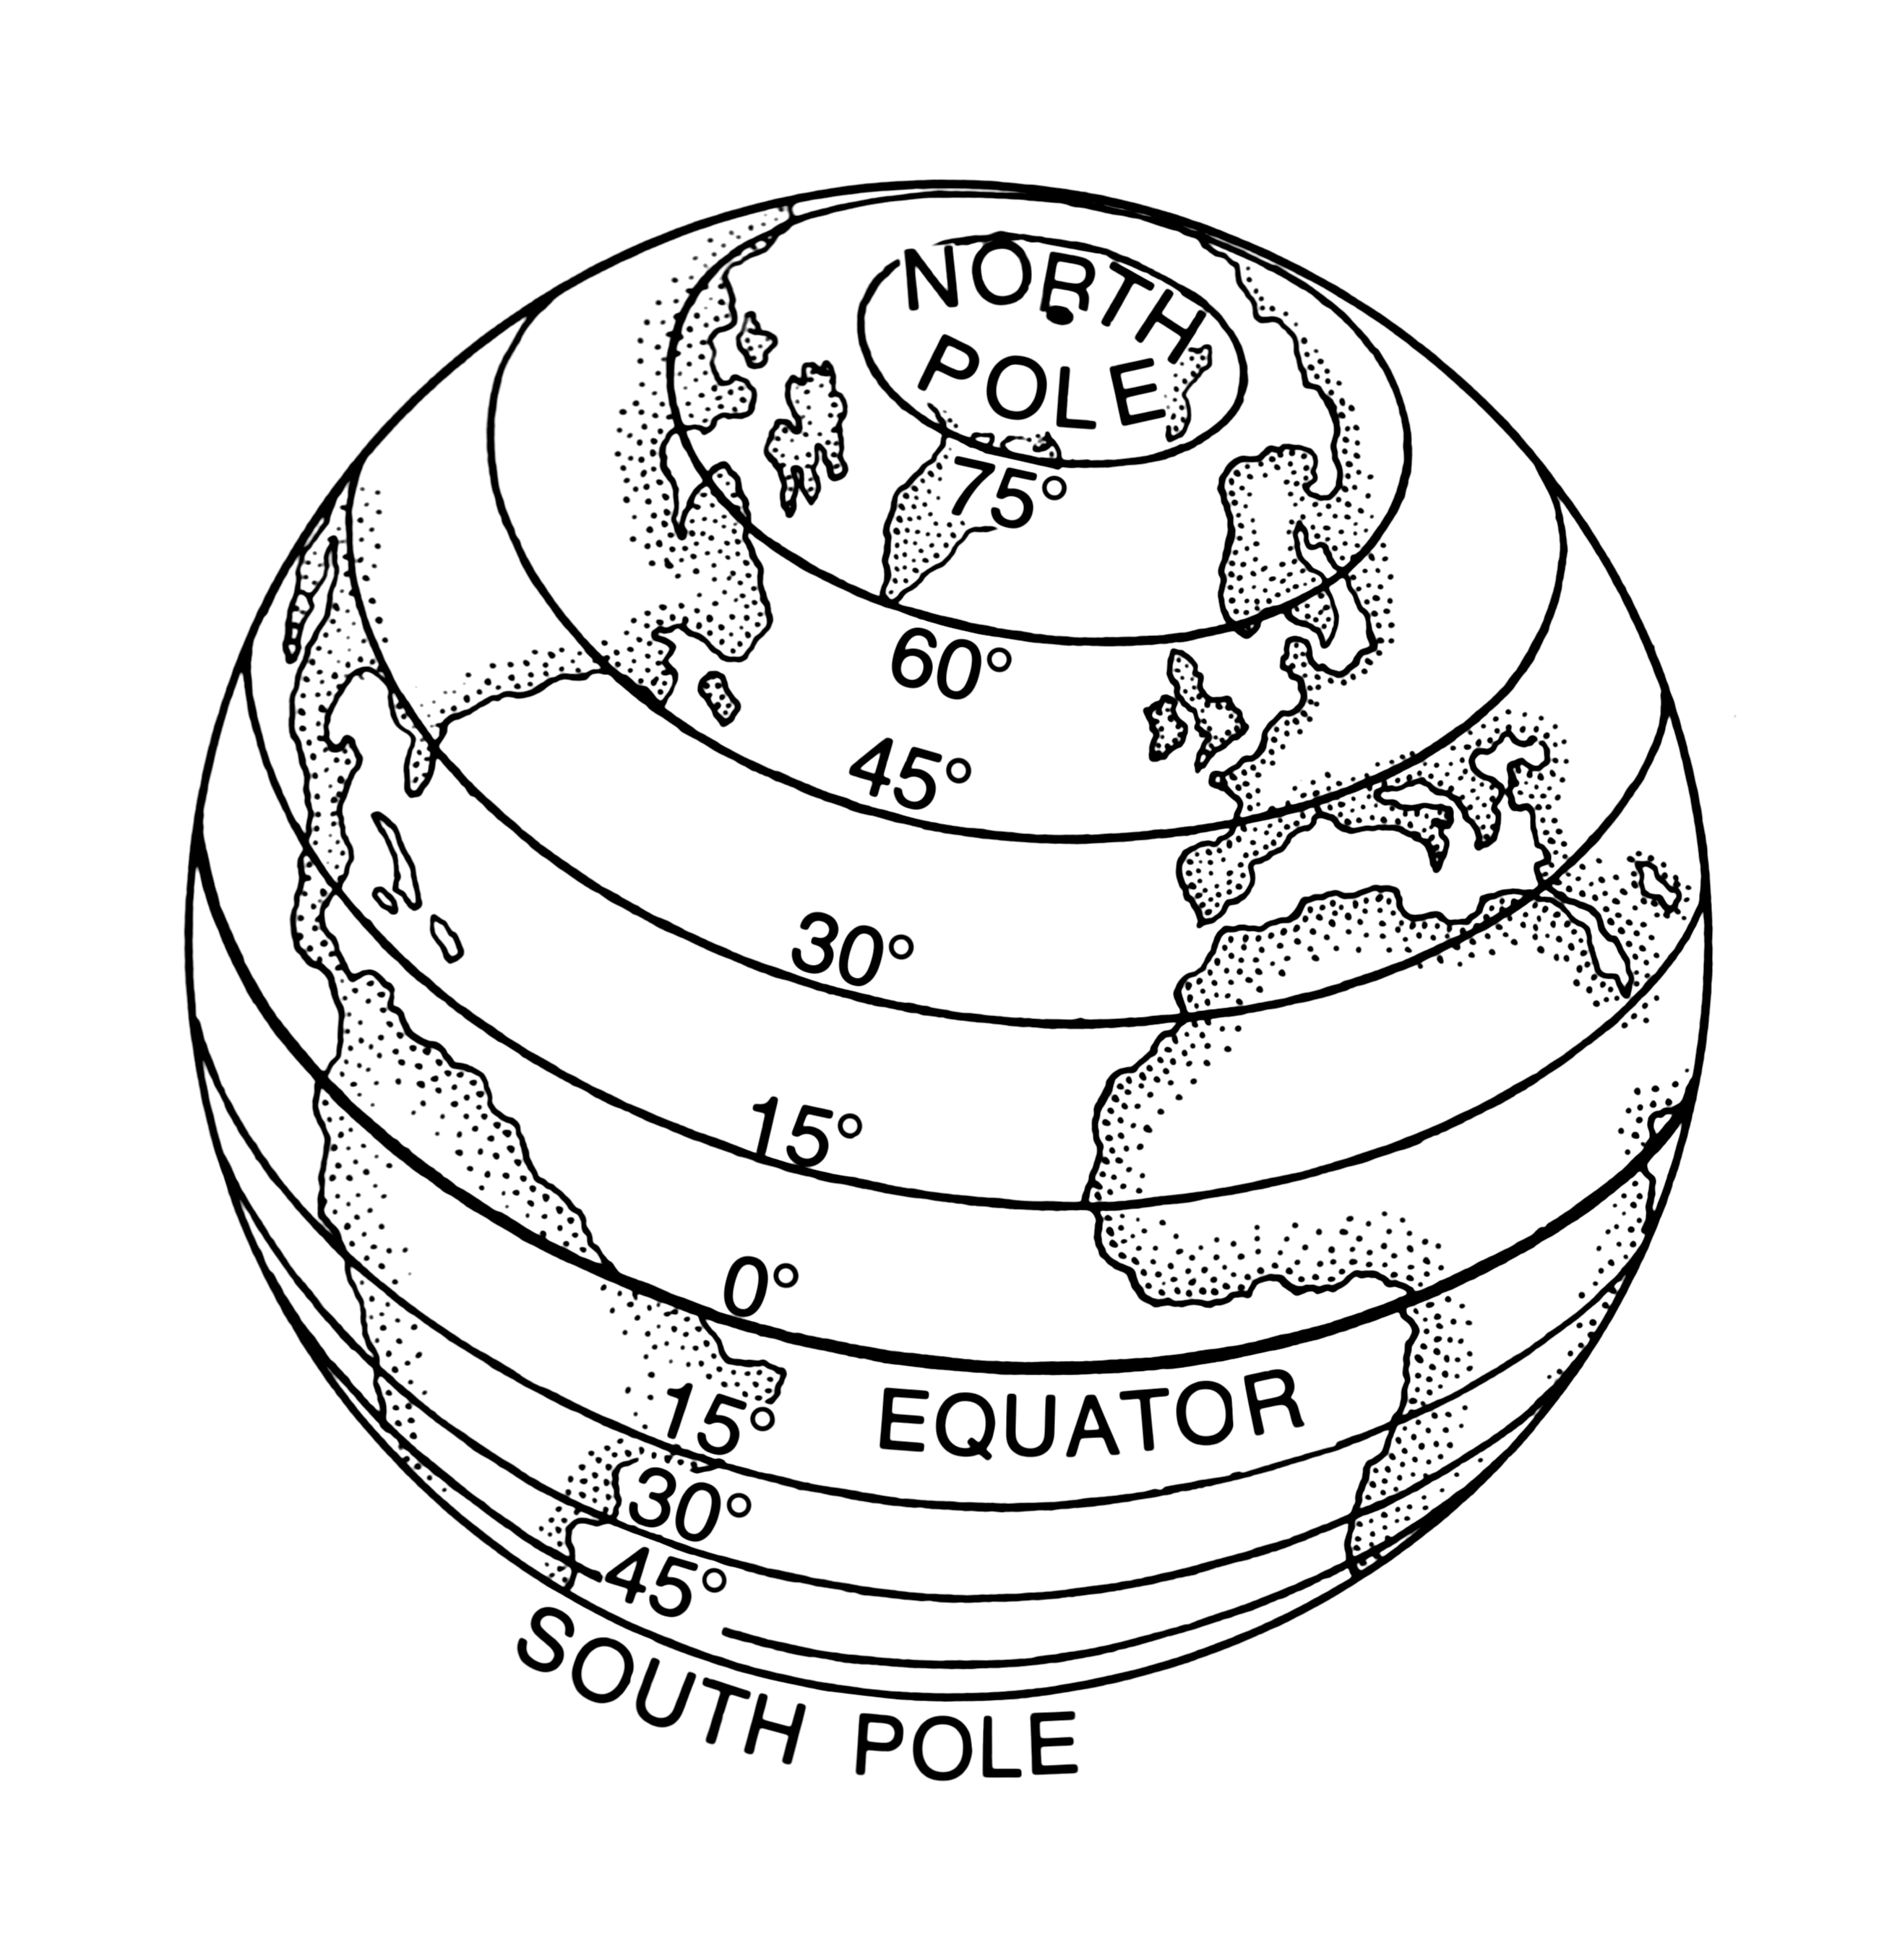
\includegraphics[width=2in]{./RadianMeasureGraphics/Latitude_(PSF).png}

&

\begin{mfpic}[18]{-5}{5}{-4}{4.75}
\axes
\tlabel(4.75,-0.5){\scriptsize $x$}
\tlabel(0.25,4.5){\scriptsize $y$}
\tlabel(3.1,-0.75){\scriptsize $3960$}
\tlabel(0.25,3.1){\scriptsize $3960$}
\tlabel(2.5, 1.75){\scriptsize $Q\left(x,y\right)$}
\tlabel(1.2, 0.15){\scriptsize $41.628^{\circ}$}
\tcaption{}
\xmarks{-3 step 3 until 3}
\ymarks{-3 step 3 until 3}
\drawcolor[gray]{0.7}
\circle{(0,0),3}
\drawcolor{black}
\dotted \polyline{(0, 1.993), (2.242, 1.993)}
\arrow \parafcn{5, 35, 5}{dir(t)}
\tcaption{A point on the Earth at $41.628^{\circ}$N}
\penwd{1.25pt}
 \arrow \reverse \arrow \polyline{(5,0), (0,0), (3.737, 3.321)}
\point[4pt]{(0,0),(2.242, 1.993)}
\end{mfpic}

\end{tabular}

\end{enumerate}

Assuming the Earth is a sphere of radius $3960$ miles, a cross-section through the poles produces a circle of radius $3960$ miles. Viewing the Equator as the $x$-axis, the value we seek is the $x$-coordinate of the point $Q(x,y)$ indicated in the figure above on the right.  Using Theorem \ref{cosinesinecircle}, we get $x = 3960 \cos\left(41.628^{\circ}\right) \approx 2960$.  Hence, the radius of the Earth at North Latitude $41.628^{\circ}$ is approximately $2960$ miles. \qed

\end{ex}
 



Theorem \ref{cosinesinecircle} gives us what we need to `circle back' to the question posed at the the beginning of the section:  how to describe the position of an object traveling in a circular path of radius $r$ with constant angular velocity $\omega$.  Suppose that at time $t$, the object has swept out an angle measuring $\theta$ radians.  If we assume that the object is at the point $(r,0)$ when $t=0$, the angle $\theta$ is in standard position.  By definition, $\omega = \frac{\theta}{t}$ which we rewrite as  $\theta = \omega t$.  According to Theorem \ref{cosinesinecircle}, the location of the object $Q(x,y)$ on the circle is found using the equations  $x = r \cos(\theta) = r \cos(\omega t)$ and $y = r \sin(\theta) = r \sin(\omega t)$.  Hence, at time $t$, the object is at the point $(r \cos(\omega t), r \sin(\omega t))$, as seen in the diagram below.

\begin{center}

\hspace{.55in} \begin{mfpic}[15]{-5}{5}{-5}{5}
\axes
\tlabel(4.75,-0.5){\scriptsize $x$}
\tlabel(0.25,4.75){\scriptsize $y$}
\tlabel(2.1,-0.75){\scriptsize $1$}
\tlabel(0.25,2.1){\scriptsize $1$}
\tlabel(4.1,-0.75){\scriptsize $r$}
\tlabel(0.25,4.1){\scriptsize $r$}
\tlabel(2.35, 3.5){\small $Q\left(x,y\right) = (r \cos(\omega t), r \sin(\omega t))$}
\xmarks{-4 step 2 until 4}
\ymarks{-4 step 2 until 4}
\drawcolor[gray]{0.7}
\circle{(0,0),4}
\drawcolor{black}
\arrow \reverse \arrow \polyline{(5,0),(0,0), (2.5, 4.3301)}
\arrow \parafcn{5, 55, 5}{dir(t)}
\tlabel[cc](1.95, .5){\small $\theta = \omega t$}
\point[4pt]{(0,0),  (2, 3.4641)}
\penwd{1.5pt}
\arrow \parafcn{0, 60, 5}{4*dir(t)}
\end{mfpic} 

\hspace{-.7in} Equations for Circular Motion

\end{center}



 We have just argued the following.


\smallskip

\colorbox{ResultColor}{\bbm
\begin{eqn} \label{equationsforcircularmotion} Suppose an object is traveling in a circular path of radius $r$ centered at the origin with constant angular velocity $\omega$.  If $t=0$ corresponds to the point $(r,0)$, then the $x$ and $y$ coordinates of the object are functions of $t$ and are given by $x =  r \cos(\omega t)$ and $y = r \sin(\omega t)$.  Here, $\omega > 0$ indicates a counter-clockwise direction and $\omega < 0$ indicates a clockwise direction.

\end{eqn}
\ebm}
\smallskip

\begin{ex}  Suppose we are in the situation of Example \ref{EarthRotationEx}.  Find the equations of motion of Lakeland Community College as the earth rotates.
\label{Lakelandrotates}

\smallskip

{\bf Solution.}  From Example \ref{EarthRotationEx}, we take $r = 2960$ miles and and $\omega = \frac{\pi}{12 \, \text{hours}}$.  Hence, the equations of motion are $x =  r \cos(\omega t) = 2960 \cos\left(\frac{\pi}{12} t\right)$ and  $y =  r \sin(\omega t) = 2960 \sin\left(\frac{\pi}{12} t\right)$, where $x$ and $y$ are measured in miles and $t$ is measured in hours.\footnote{We will revisit this concept of associating points with times in Section \ref{ParametricEquations}.} \qed

\end{ex}




\newpage

\subsection{Exercises}

\documentclass{ximera}

\begin{document}
	\author{Stitz-Zeager}
	\xmtitle{TITLE}



In Exercises \ref{valuefirst} - \ref{valuelast}, find the exact value of the cosine and sine of the given angle.

\begin{multicols}{4}

\begin{enumerate}

\item $\theta = 0$ \vphantom{$\dfrac{\pi}{4}$} \label{valuefirst}
\item $\theta = \dfrac{\pi}{4}$
\item $\theta = \dfrac{\pi}{3}$
\item $\theta = \dfrac{\pi}{2}$

\setcounter{HW}{\value{enumi}}

\end{enumerate}

\end{multicols}

\begin{multicols}{4}

\begin{enumerate}

\setcounter{enumi}{\value{HW}}

\item $\theta = \dfrac{2\pi}{3}$
\item $\theta = \dfrac{3\pi}{4}$
\item $\theta = \pi$ \vphantom{$\dfrac{7\pi}{4}$}
\item $\theta = \dfrac{7\pi}{6}$

\setcounter{HW}{\value{enumi}}

\end{enumerate}

\end{multicols}

\begin{multicols}{4}

\begin{enumerate}

\setcounter{enumi}{\value{HW}}

\item $\theta = \dfrac{5\pi}{4}$
\item $\theta = \dfrac{4\pi}{3}$
\item $\theta = \dfrac{3\pi}{2}$
\item $\theta = \dfrac{5\pi}{3}$

\setcounter{HW}{\value{enumi}}

\end{enumerate}

\end{multicols}

\begin{multicols}{4}

\begin{enumerate}

\setcounter{enumi}{\value{HW}}

\item $\theta = \dfrac{7\pi}{4}$
\item $\theta = \dfrac{23\pi}{6}$
\item $\theta = -\dfrac{13\pi}{2}$
\item $\theta = -\dfrac{43\pi}{6}$

\setcounter{HW}{\value{enumi}}

\end{enumerate}

\end{multicols}

\begin{multicols}{4}

\begin{enumerate}

\setcounter{enumi}{\value{HW}}

\item $\theta = -\dfrac{3\pi}{4}$
\item $\theta = -\dfrac{\pi}{6}$ \vphantom{$\dfrac{7\pi}{4}$}
\item $\theta = \dfrac{10\pi}{3}$
\item $\theta = 117\pi$ \vphantom{$\dfrac{7\pi}{4}$} \label{valuelast}

\setcounter{HW}{\value{enumi}}

\end{enumerate}

\end{multicols}

In Exercises \ref{solveforanglefirst} - \ref{solveforanglelast}, find all of the angles which satisfy the given equation.

\begin{multicols}{3}

\begin{enumerate}

\setcounter{enumi}{\value{HW}}

\item $\sin(\theta) = \dfrac{1}{2}$ \vphantom{$\dfrac{2}{2}$} \label{solveforanglefirst}
\item $\cos(\theta) = -\dfrac{\sqrt{3}}{2}$
\item $\sin(\theta) = 0$ \vphantom{$\dfrac{2}{2}$}

\setcounter{HW}{\value{enumi}}

\end{enumerate}

\end{multicols}

\begin{multicols}{3}

\begin{enumerate}

\setcounter{enumi}{\value{HW}}

\item $\cos(\theta) = \dfrac{\sqrt{2}}{2}$
\item $\sin(\theta) = \dfrac{\sqrt{3}}{2}$
\item $\cos(\theta) = -1$ \vphantom{$\dfrac{\sqrt{2}}{2}$}

\setcounter{HW}{\value{enumi}}

\end{enumerate}

\end{multicols}

\begin{multicols}{3}

\begin{enumerate}

\setcounter{enumi}{\value{HW}}

\item  $\sin(\theta) = -1$ \vphantom{$\dfrac{\sqrt{2}}{2}$}
\item  $\cos(\theta) = \dfrac{\sqrt{3}}{2}$
\item  $\cos(\theta) = -1.001$ \vphantom{$\dfrac{\sqrt{2}}{2}$} \label{solveforanglelast}

\setcounter{HW}{\value{enumi}}

\end{enumerate}

\end{multicols}

In Exercises \ref{solvefortfirst} - \ref{solvefortlast}, solve the equation for $t$.  (See the remarks on page \ref{cosinesineequationsrealnumbers}.)

\begin{multicols}{3}

\begin{enumerate}

\setcounter{enumi}{\value{HW}}

\item $\cos(t) = 0$ \vphantom{$\dfrac{\sqrt{2}}{2}$} \label{solvefortfirst}
\item $\sin(t) = -\dfrac{\sqrt{2}}{2}$
\item $\cos(t) = 3$ \vphantom{$\dfrac{\sqrt{2}}{2}$}

\setcounter{HW}{\value{enumi}}

\end{enumerate}

\end{multicols}

\begin{multicols}{3}

\begin{enumerate}

\setcounter{enumi}{\value{HW}}

\item $\sin(t) = -\dfrac{1}{2}$
\item $\cos(t) = \dfrac{1}{2}$
\item $\sin(t) = -2$ \vphantom{$\dfrac{1}{2}$}

\setcounter{HW}{\value{enumi}}

\end{enumerate}

\end{multicols}

\begin{multicols}{3}

\begin{enumerate}

\setcounter{enumi}{\value{HW}}

\item $\cos(t) = 1$ \vphantom{$\dfrac{\sqrt{2}}{2}$}
\item $\sin(t) = 1$ \vphantom{$\dfrac{\sqrt{2}}{2}$}
\item $\cos(t) = -\dfrac{\sqrt{2}}{2}$ \label{solvefortlast}

\setcounter{HW}{\value{enumi}}

\end{enumerate}

\end{multicols}

In Exercises \ref{pointsfirst} - \ref{pointslast}, let $\theta$ be the angle in standard position whose terminal side contains the given point then compute $\cos(\theta)$ and $\sin(\theta)$.

\begin{multicols}{4}

\begin{enumerate}

\setcounter{enumi}{\value{HW}}

\item $P(-7, 24)$ \label{pointsfirst} 
\item $Q(3, 4)$
\item $R(5, -9)$
\item $T(-2, -11)$ \label{pointslast}

\setcounter{HW}{\value{enumi}}

\end{enumerate}

\end{multicols}

\newpage

In Exercises \ref{findthevaluefirst} - \ref{findthevaluelast}, use the results developed throughout the section to find the requested value.

\begin{enumerate}

\setcounter{enumi}{\value{HW}}

\item If $\sin(\theta) = -\dfrac{7}{25}$ with $\theta$ in Quadrant IV, what is $\cos(\theta)$? \label{findthevaluefirst}
\item If $\cos(\theta) = \dfrac{4}{9}$ with $\theta$ in Quadrant I, what is $\sin(\theta)$?
\item If $\sin(\theta) = \dfrac{5}{13}$ with $\theta$ in Quadrant II, what is $\cos(\theta)$?
\item If $\cos(\theta) = -\dfrac{2}{11}$ with $\theta$ in Quadrant III, what is $\sin(\theta)$?
\item If $\sin(\theta) = -\dfrac{2}{3}$ with $\theta$ in Quadrant III, what is $\cos(\theta)$?
\item If $\cos(\theta) = \dfrac{28}{53}$ with $\theta$ in Quadrant IV, what is $\sin(\theta)$?
\item  If $\sin(\theta) = \dfrac{2\sqrt{5}}{5}$ and $\dfrac{\pi}{2} < \theta < \pi$, what is $\cos(\theta)$?
\item  If $\cos(\theta) = \dfrac{\sqrt{10}}{10}$ and $2\pi < \theta < \dfrac{5\pi}{2}$, what is $\sin(\theta)$?
\item  If $\sin(\theta) = -0.42$ and $\pi < \theta < \dfrac{3\pi}{2}$, what is  $\cos(\theta)$?
\item  If $\cos(\theta) = -0.98$ and $\dfrac{\pi}{2} < \theta < \pi$, what is $\sin(\theta)$? \label{findthevaluelast}

\setcounter{HW}{\value{enumi}}

\end{enumerate}

In Exercises \ref{calculatorfirst} - \ref{calculatorlast}, use your calculator to approximate the given value to three decimal places.  Make sure your calculator is in the proper angle measurement mode!

\begin{multicols}{3}

\begin{enumerate}

\setcounter{enumi}{\value{HW}}

\item $\sin(78.95^{\circ})$ \label{calculatorfirst}
\item $\cos(-2.01)$
\item $\sin(392.994)$

\setcounter{HW}{\value{enumi}}

\end{enumerate}

\end{multicols}

\begin{multicols}{3}

\begin{enumerate}

\setcounter{enumi}{\value{HW}}

\item $\cos(207^{\circ})$
\item $\sin\left( \pi^{\circ} \right)$
\item $\cos(e)$ \label{calculatorlast} 

\setcounter{HW}{\value{enumi}}

\end{enumerate}

\end{multicols}

In Exercises \ref{decomposebasicsinecosinefirst} - \ref{decomposebasicsinecosinelast}, write the given function as a nontrivial decomposition of functions as directed.

\begin{enumerate}
\setcounter{enumi}{\value{HW}}

\item  For $f(t) = 3t + \sin(2t)$, find functions $g$ and $h$ so that $f=g+h$. \label{decomposebasicsinecosinefirst}
\item  For $f(\theta) = 3\cos(\theta) - \sin(4\theta)$, find functions $g$ and $h$ so that $f=g-h$. 
\item  For $f(t) = e^{-0.1t} \sin(3t)$, find functions $g$ and $h$ so that $f=gh$.
\item  For $r(t) = \dfrac{\sin(t)}{t}$, find functions $f$ and $g$ so $r = \dfrac{f}{g}$.
\item  For $r(\theta) =\sqrt{3 \cos(\theta)}$, find functions $f$ and $g$ so $r = g \circ f$. \label{decomposebasicsinecosinelast}

\setcounter{HW}{\value{enumi}}
\end{enumerate}

\begin{enumerate}
\setcounter{enumi}{\value{HW}}

\item \label{sinearcexercise}For each function $S(t)$ listed below, compute the average rate of change over the indicated interval.\footnote{See Definition \ref{arc} in Section \ref{AverageRateofChange} for a review of this concept, as needed.}  What trends do you notice? Be sure your calculator is in radian mode!

\[ \begin{array}{|r||c|c|c|}  \hline

 S(t) &  [-0.1, 0.1] & [-0.01, 0.01] &[-0.001, 0.001] \\ \hline
 \sin(t)     &&&  \\  \hline
 \sin(2t)   &&&  \\ \hline
 \sin(3t)   &&&   \\  \hline
\sin(4t)   &&&   \\  \hline

\end{array} \]

\setcounter{HW}{\value{enumi}}
\end{enumerate}

In Exercises \ref{motionfirst} - \ref{motionlast}, find the equations of motion for the given scenario.  Assume that the center of the motion is the origin, the motion is counter-clockwise and that $t = 0$ corresponds to a position along the positive $x$-axis.  (See Equation \ref{equationsforcircularmotion} and Example \ref{EarthRotationEx}.)

\begin{enumerate}

\setcounter{enumi}{\value{HW}}

\item  \label{motionfirst} A point on the edge of the spinning yo-yo in Exercise \ref{spinningyoyo} from Section \ref{RadianMeasure}. 

Recall: The diameter of the yo-yo is 2.25 inches and it spins at 4500 revolutions per minute.

\item  The yo-yo in exercise \ref{yoyotrick} from Section \ref{RadianMeasure}.

Recall: The radius of the circle is 28 inches and it completes one revolution in 3 seconds.

\item A point on the edge of the hard drive in Exercise \ref{harddrive} from Section \ref{RadianMeasure}.

Recall:  The diameter of the hard disk is 2.5 inches and it spins at 7200 revolutions per minute.

\item  \label{motionlast} A passenger on the Big Wheel in Exercise \ref{giantwheelmotion} from Section \ref{RadianMeasure}.

Recall: The diameter is 128 feet and completes 2 revolutions in 2 minutes, 7 seconds.

\setcounter{HW}{\value{enumi}}

\end{enumerate}

\begin{enumerate}

\setcounter{enumi}{\value{HW}}

\item Consider the numbers:  $0$, $1$, $2$, $3$, $4$.  Take the square root of each of these numbers, then divide each by $2$. The resulting numbers should look hauntingly familiar. (See the values in the table on \pageref{CosineSineFacts}.) 


\item  On page \pageref{cosinesineequationsrealnumbers}, we see that the sine and cosine functions of \textit{angles} can be considered functions of \textit{real numbers}.  With help from your classmates, discuss the domains and ranges of  $f(t) = \sin(t)$ and $g(t) = \cos(t)$.  Write your answers using interval notation.


\item  \label{circleofradiusrsinecosinetrans}  Another way to establish  Theorem \ref{cosinesinecircle} is to use transformations. Re-read the discussion following  Theorem \ref{standardcirclealternate} in Chapter \ref{TheConicSections}  and transform  the Unit Circle, $x^2+y^2 = 1$, to $x^2 + y^2 = r^2$ using horizontal and vertical stretches.  Show if the coordinates on the Unit Circle are $(\cos(\theta), \sin(\theta))$, then the corresponding coordinates on $x^2+y^2 = r^2$ are $(r \cos(\theta), r \sin(\theta))$.

\item  In the scenario of Equation \ref{equationsforcircularmotion}, we assumed that at $t=0$, the object was at the point $(r,0)$.  If this is not the case,  we can adjust the equations of motion by introducing a `time delay.'   If $t_{0} > 0$ is the first time the object passes through the point $(r,0)$, show, with the help of your classmates, the equations of motion are $x = r \cos(\omega (t - t_{0}))$ and $y = r \sin(\omega (t-t_{0}))$.


\end{enumerate}

\newpage

\subsection{Answers}

\begin{multicols}{2}

\begin{enumerate}

\item $\cos(0) = 1$, $\; \sin(0) = 0$ \vphantom{$\dfrac{\sqrt{2}}{2}$}

\item $\cos \left(\dfrac{\pi}{4} \right) = \dfrac{\sqrt{2}}{2}$, $\; \sin \left(\dfrac{\pi}{4} \right) = \dfrac{\sqrt{2}}{2}$

\setcounter{HW}{\value{enumi}}

\end{enumerate}

\end{multicols}

\begin{multicols}{2}

\begin{enumerate}

\setcounter{enumi}{\value{HW}}

\item $\cos \left(\dfrac{\pi}{3}\right) = \dfrac{1}{2}$, $\; \sin \left(\dfrac{\pi}{3}\right) = \dfrac{\sqrt{3}}{2}$

\item $\cos \left(\dfrac{\pi}{2}\right) = 0$, $\; \sin \left(\dfrac{\pi}{2}\right) = 1$ \vphantom{$\dfrac{\sqrt{2}}{2}$}

\setcounter{HW}{\value{enumi}}

\end{enumerate}

\end{multicols}

\begin{multicols}{2}

\begin{enumerate}

\setcounter{enumi}{\value{HW}}

\item $\cos\left(\dfrac{2\pi}{3}\right) = -\dfrac{1}{2}$, $\; \sin \left(\dfrac{2\pi}{3}\right) = \dfrac{\sqrt{3}}{2}$

\item $\cos \left(\dfrac{3\pi}{4} \right) = -\dfrac{\sqrt{2}}{2}$, $\; \sin \left(\dfrac{3\pi}{4} \right) = \dfrac{\sqrt{2}}{2}$

\setcounter{HW}{\value{enumi}}

\end{enumerate}

\end{multicols}

\begin{multicols}{2}

\begin{enumerate}

\setcounter{enumi}{\value{HW}}

\item $\cos(\pi) = -1$, $\; \sin(\pi) = 0$ \vphantom{$\dfrac{\sqrt{3}}{2}$}

\item $\cos\left(\dfrac{7\pi}{6}\right) = -\dfrac{\sqrt{3}}{2}$, $\; \sin\left(\dfrac{7\pi}{6}\right) = -\dfrac{1}{2}$

\setcounter{HW}{\value{enumi}}

\end{enumerate}

\end{multicols}

\begin{multicols}{2}

\begin{enumerate}

\setcounter{enumi}{\value{HW}}

\item $\cos \left(\dfrac{5\pi}{4} \right) = -\dfrac{\sqrt{2}}{2}$, $\; \sin \left(\dfrac{5\pi}{4} \right) = -\dfrac{\sqrt{2}}{2}$

\item $\cos\left(\dfrac{4\pi}{3}\right) = -\dfrac{1}{2}$, $\; \sin \left(\dfrac{4\pi}{3}\right) = -\dfrac{\sqrt{3}}{2}$

\setcounter{HW}{\value{enumi}}

\end{enumerate}

\end{multicols}

\begin{multicols}{2}

\begin{enumerate}

\setcounter{enumi}{\value{HW}}

\item $\cos \left(\dfrac{3\pi}{2}\right) = 0$, $\; \sin \left(\dfrac{3\pi}{2}\right) = -1$

\item $\cos\left(\dfrac{5\pi}{3}\right) = \dfrac{1}{2}$, $\; \sin \left(\dfrac{5\pi}{3}\right) = -\dfrac{\sqrt{3}}{2}$

\setcounter{HW}{\value{enumi}}

\end{enumerate}

\end{multicols}

\begin{multicols}{2}

\begin{enumerate}

\setcounter{enumi}{\value{HW}}

\item $\cos \left(\dfrac{7\pi}{4} \right) = \dfrac{\sqrt{2}}{2}$, $\; \sin \left(\dfrac{7\pi}{4} \right) = -\dfrac{\sqrt{2}}{2}$

\item $\cos\left(\dfrac{23\pi}{6}\right) = \dfrac{\sqrt{3}}{2}$, $\; \sin\left(\dfrac{23\pi}{6}\right) = -\dfrac{1}{2}$

\setcounter{HW}{\value{enumi}}

\end{enumerate}

\end{multicols}

\begin{multicols}{2}

\begin{enumerate}

\setcounter{enumi}{\value{HW}}

\item $\cos \left(-\dfrac{13\pi}{2}\right) = 0$, $\; \sin \left(-\dfrac{13\pi}{2}\right) = -1$ \vphantom{$\dfrac{\sqrt{3}}{2}$}

\item $\cos\left(-\dfrac{43\pi}{6}\right) = -\dfrac{\sqrt{3}}{2}$, $\; \sin\left(-\dfrac{43\pi}{6}\right) = \dfrac{1}{2}$

\setcounter{HW}{\value{enumi}}

\end{enumerate}

\end{multicols}

\begin{multicols}{2}

\begin{enumerate}

\setcounter{enumi}{\value{HW}}

\item $\cos \left(-\dfrac{3\pi}{4} \right) = -\dfrac{\sqrt{2}}{2}$, $\; \sin \left(-\dfrac{3\pi}{4} \right) = -\dfrac{\sqrt{2}}{2}$

\item $\cos\left(-\dfrac{\pi}{6}\right) = \dfrac{\sqrt{3}}{2}$, $\; \sin\left(-\dfrac{\pi}{6}\right) = -\dfrac{1}{2}$

\setcounter{HW}{\value{enumi}}

\end{enumerate}

\end{multicols}

\begin{multicols}{2}

\begin{enumerate}

\setcounter{enumi}{\value{HW}}

\item $\cos\left(\dfrac{10\pi}{3}\right) = -\dfrac{1}{2}$, $\; \sin \left(\dfrac{10\pi}{3}\right) = -\dfrac{\sqrt{3}}{2}$

\item $\cos(117\pi) = -1$, $\; \sin(117\pi) = 0$ \vphantom{$\dfrac{\sqrt{3}}{2}$}

\setcounter{HW}{\value{enumi}}

\end{enumerate}

\end{multicols}

\begin{enumerate}

\setcounter{enumi}{\value{HW}}

\item $\sin(\theta) = \dfrac{1}{2}$ when $\theta = \dfrac{\pi}{6} + 2\pi k$ or $\theta = \dfrac{5\pi}{6} + 2\pi k$ for any integer $k$.
\item $\cos(\theta) = -\dfrac{\sqrt{3}}{2}$ when $\theta = \dfrac{5\pi}{6} + 2\pi k$ or $\theta = \dfrac{7\pi}{6} + 2\pi k$ for any integer $k$.
\item $\sin(\theta) = 0$ when $\theta = \pi k$ for any integer $k$.
\item $\cos(\theta) = \dfrac{\sqrt{2}}{2}$ when $\theta = \dfrac{\pi}{4} + 2\pi k$ or $\theta = \dfrac{7\pi}{4} + 2\pi k$ for any integer $k$.
\item $\sin(\theta) = \dfrac{\sqrt{3}}{2}$ when $\theta = \dfrac{\pi}{3} + 2\pi k$ or $\theta = \dfrac{2\pi}{3} + 2\pi k$ for any integer $k$.
\item $\cos(\theta) = -1$ when $\theta = (2k + 1)\pi$ for any integer $k$.
\item  $\sin(\theta) = -1$ when $\theta = \dfrac{3\pi}{2} + 2\pi k$ for any integer $k$.
\item  $\cos(\theta) = \dfrac{\sqrt{3}}{2}$ when $\theta = \dfrac{\pi}{6} + 2\pi k$ or  $\theta = \dfrac{11\pi}{6} + 2\pi k$ for any integer $k$.
%\item  $\sin(\theta) = \dfrac{\sqrt{2}}{2}$ when $\theta = \dfrac{\pi}{4} + 2\pi k$ or  $\theta = \dfrac{3\pi}{4} + 2\pi k$ for any integer $k$.
\item  $\cos(\theta) = -1.001$ never happens

\setcounter{HW}{\value{enumi}}

\end{enumerate}

\begin{enumerate}

\setcounter{enumi}{\value{HW}}

\item $\cos(t) = 0$ when $t = \dfrac{\pi}{2} + \pi k$ for any integer $k$.
\item $\sin(t) = -\dfrac{\sqrt{2}}{2}$ when $t = \dfrac{5\pi}{4} + 2\pi k$ or $t = \dfrac{7\pi}{4} + 2\pi k$ for any integer $k$.
\item $\cos(t) = 3$ never happens.  
\item $\sin(t) = -\dfrac{1}{2}$ when $t = \dfrac{7\pi}{6} + 2\pi k$ or $t = \dfrac{11\pi}{6} + 2\pi k$ for any integer $k$.
\item $\cos(t) = \dfrac{1}{2}$ when $t = \dfrac{\pi}{3} + 2\pi k$ or $t = \dfrac{5\pi}{3} + 2\pi k$ for any integer $k$.
\item $\sin(t) = -2$ never happens
\item $\cos(t) = 1$ when $t = 2\pi k$ for any integer $k$.
\item $\sin(t) = 1$ when $t = \dfrac{\pi}{2} + 2\pi k$ for any integer $k$.
\item $\cos(t) = -\dfrac{\sqrt{2}}{2}$ when $t = \dfrac{3\pi}{4} + 2\pi k$ or $t = \dfrac{5\pi}{4} + 2\pi k$ for any integer $k$.
%\item  $\sin(t) = -\dfrac{\sqrt{3}}{2}$ when $t = \dfrac{4\pi}{3} + 2\pi k$ or  $t = \dfrac{5\pi}{3} + 2\pi k$ for any integer $k$.

\setcounter{HW}{\value{enumi}}

\end{enumerate}

\begin{enumerate}

\setcounter{enumi}{\value{HW}}

\item $\cos(\theta) = -\dfrac{7}{25}, \; \sin(\theta) = \dfrac{24}{25}$

\item $\cos(\theta) = \dfrac{3}{5}, \; \sin(\theta) = \dfrac{4}{5}$

\item $\cos(\theta) = \dfrac{5\sqrt{106}}{106}, \; \sin(\theta) = -\dfrac{9\sqrt{106}}{106}$

\item $\cos(\theta) = -\dfrac{2\sqrt{5}}{25}, \; \sin(\theta) = -\dfrac{11\sqrt{5}}{25}$

\setcounter{HW}{\value{enumi}}

\end{enumerate}


\begin{enumerate}

\setcounter{enumi}{\value{HW}}

\item If $\sin(\theta) = -\dfrac{7}{25}$ with $\theta$ in Quadrant IV, then $\cos(\theta) = \dfrac{24}{25}$.
\item If $\cos(\theta) = \dfrac{4}{9}$ with $\theta$ in Quadrant I, then $\sin(\theta) = \dfrac{\sqrt{65}}{9}$.
\item If $\sin(\theta) = \dfrac{5}{13}$ with $\theta$ in Quadrant II, then $\cos(\theta) = -\dfrac{12}{13}$.
\item If $\cos(\theta) = -\dfrac{2}{11}$ with $\theta$ in Quadrant III, then $\sin(\theta) = -\dfrac{\sqrt{117}}{11}$.
\item If $\sin(\theta) = -\dfrac{2}{3}$ with $\theta$ in Quadrant III, then $\cos(\theta) = -\dfrac{\sqrt{5}}{3}$.
\item If $\cos(\theta) = \dfrac{28}{53}$ with $\theta$ in Quadrant IV, then $\sin(\theta) = -\dfrac{45}{53}$.
\item  If $\sin(\theta) = \dfrac{2\sqrt{5}}{5}$ and $\dfrac{\pi}{2} < \theta < \pi$, then $\cos(\theta) = -\dfrac{\sqrt{5}}{5}$.
\item  If $\cos(\theta) = \dfrac{\sqrt{10}}{10}$ and $2\pi < \theta < \dfrac{5\pi}{2}$, then $\sin(\theta)  = \dfrac{3 \sqrt{10}}{10}$.
\item  If $\sin(\theta) = -0.42$ and $\pi < \theta < \dfrac{3\pi}{2}$, then $\cos(\theta) = -\sqrt{0.8236} \approx -0.9075$.
\item  If $\cos(\theta) = -0.98$ and $\dfrac{\pi}{2} < \theta < \pi$, then $\sin(\theta) = \sqrt{0.0396} \approx 0.1990$.

\setcounter{HW}{\value{enumi}}

\end{enumerate}


\begin{multicols}{3}

\begin{enumerate}

\setcounter{enumi}{\value{HW}}

\item $\sin(78.95^{\circ}) \approx 0.981$
\item $\cos(-2.01) \approx -0.425$
\item $\sin(392.994) \approx -0.291$

\setcounter{HW}{\value{enumi}}

\end{enumerate}

\end{multicols}

\begin{multicols}{3}

\begin{enumerate}

\setcounter{enumi}{\value{HW}}

\item $\cos(207^{\circ}) \approx -0.891$
\item $\sin\left( \pi^{\circ} \right) \approx 0.055$
\item $\cos(e) \approx -0.912$

\setcounter{HW}{\value{enumi}}

\end{enumerate}
\end{multicols}

\begin{enumerate}
\setcounter{enumi}{\value{HW}}

\item One solution is $g(t) = 3t$ and $h(t) = \sin(2t)$.
\item One solution is $g(\theta) = 3 \cos(\theta)$ and $h(\theta) = \sin(4 \theta)$.
\item One solution is $g(t) =  e^{-0.1t}$ and $h(t) = \sin(3t)$. 
\item One solution is $f(t) = \sin(t)$ and $g(t) = t$.
\item One solution is $f(\theta) = 3 \cos(\theta)$ and $g(\theta) = \sqrt{\theta}$.

\setcounter{HW}{\value{enumi}}
\end{enumerate}

\begin{enumerate}
\setcounter{enumi}{\value{HW}}

\item  As we zoom in towards $0$, the average rate of change of $\sin(k t)$ approaches $k$.

\[ \begin{array}{|r||c|c|c|}  \hline

 S(t) &  [-0.1, 0.1] & [-0.01, 0.01] &[-0.001, 0.001] \\ \hline
 \sin(t)     & \approx 0.9983  &  \approx 1  &  \approx 1 \\  \hline
 \sin(2t)   & \approx 1.9867 & \approx  1.9999 & \approx 2 \\ \hline
 \sin(3t)   & \approx 2.9552 & \approx 2.9995 &  \approx 3  \\  \hline
 \sin(4t)  & \approx 3.8942 & \approx 3.9989 &  \approx 4 \\  \hline

\end{array} \]

\setcounter{HW}{\value{enumi}}
\end{enumerate}


\begin{enumerate}

\setcounter{enumi}{\value{HW}}

\item   $r = 1.125$ inches, $\omega = 9000 \pi \, \frac{\text{radians}}{\text{minute}}$,  $x = 1.125 \cos(9000 \pi \, t)$, $y = 1.125 \sin(9000 \pi \, t)$.  Here $x$ and $y$ are measured in inches and $t$ is measured in minutes.

\item   $r = 28$ inches, $\omega = \frac{2\pi}{3} \, \frac{\text{radians}}{\text{second}}$,  $x = 28 \cos\left(\frac{2\pi}{3} \, t \right)$, $y = 28 \sin\left(\frac{2\pi}{3} \, t \right)$.  Here $x$ and $y$ are measured in inches and $t$ is measured in seconds.

\item $r = 1.25$ inches, $\omega = 14400 \pi \, \frac{\text{radians}}{\text{minute}}$,  $x = 1.25 \cos(14400 \pi \, t)$, $y = 1.25 \sin(14400 \pi \, t)$.  Here $x$ and $y$ are measured in inches and $t$ is measured in minutes.

\item  $r = 64$ feet, $\omega = \frac{4\pi}{127} \, \frac{\text{radians}}{\text{second}}$,  $x = 64 \cos\left(\frac{4\pi}{127} \, t \right)$, $y = 64 \sin\left(\frac{4\pi}{127} \, t \right)$.  Here $x$ and $y$ are measured in feet and $t$ is measured in seconds

\end{enumerate}


\end{document}


\closegraphsfile

\end{document}
